% Graphic for TeX using PGF
% Title: C:\Users\Joan\Documents\Repos\Ken-Ken\EntregLatex\Diagrama1.dia
% Creator: Dia v0.97.2
% CreationDate: Thu Oct 08 18:14:08 2015
% For: Joan
% \usepackage{tikz}
% The following commands are not supported in PSTricks at present
% We define them conditionally, so when they are implemented,
% this pgf file will use them.
\ifx\du\undefined
  \newlength{\du}
\fi
\setlength{\du}{15\unitlength}
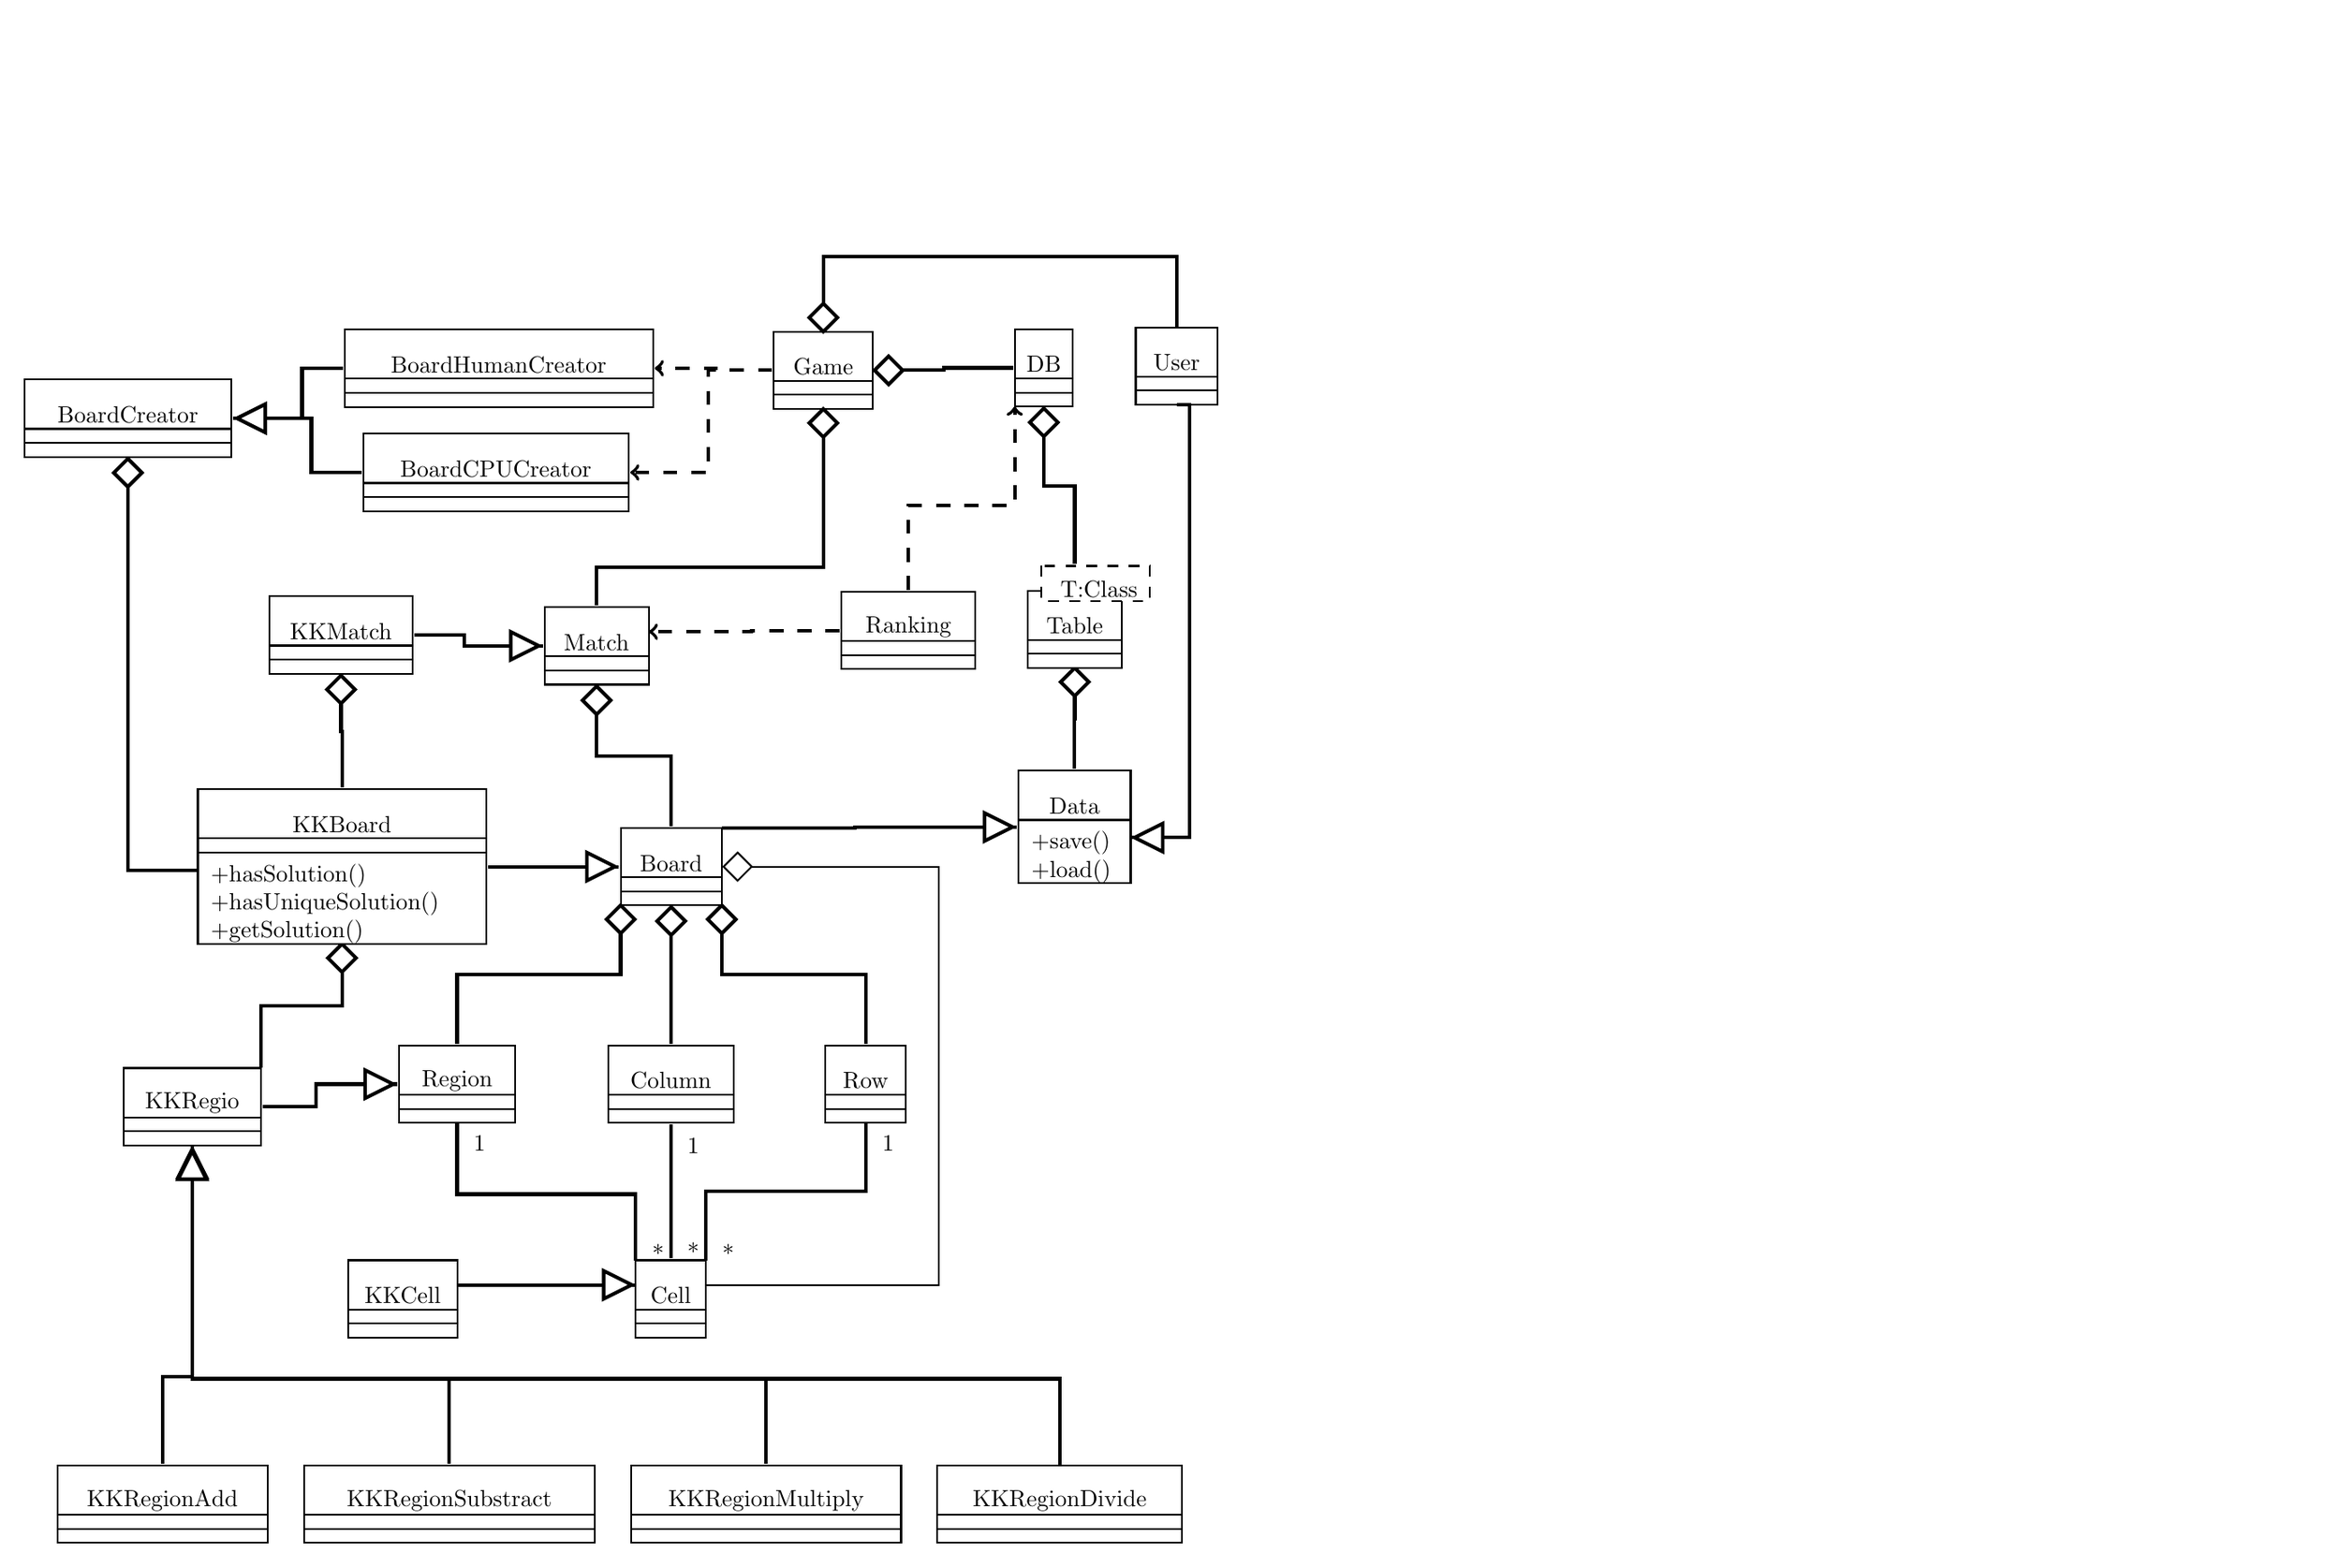
\begin{tikzpicture}
\pgftransformxscale{1.000000}
\pgftransformyscale{-1.000000}
\definecolor{dialinecolor}{rgb}{0.000000, 0.000000, 0.000000}
\pgfsetstrokecolor{dialinecolor}
\definecolor{dialinecolor}{rgb}{1.000000, 1.000000, 1.000000}
\pgfsetfillcolor{dialinecolor}
\pgfsetlinewidth{0.100000\du}
\pgfsetdash{}{0pt}
\pgfsetbuttcap
{
\definecolor{dialinecolor}{rgb}{0.000000, 0.000000, 0.000000}
\pgfsetfillcolor{dialinecolor}
% was here!!!
\definecolor{dialinecolor}{rgb}{0.000000, 0.000000, 0.000000}
\pgfsetstrokecolor{dialinecolor}
\draw (7.293010\du,21.114160\du)--(7.293010\du,18.896357\du)--(6.415651\du,18.896357\du)--(6.415651\du,16.678555\du);
}
\definecolor{dialinecolor}{rgb}{0.000000, 0.000000, 0.000000}
\pgfsetstrokecolor{dialinecolor}
\draw (7.293010\du,21.114160\du)--(7.293010\du,18.896357\du)--(6.415651\du,18.896357\du)--(6.415651\du,17.337134\du);
\pgfsetdash{}{0pt}
\pgfsetmiterjoin
\pgfsetbuttcap
\definecolor{dialinecolor}{rgb}{1.000000, 1.000000, 1.000000}
\pgfsetfillcolor{dialinecolor}
\fill (6.415651\du,16.678555\du)--(6.815651\du,17.078555\du)--(6.415651\du,17.478555\du)--(6.015651\du,17.078555\du)--cycle;
\pgfsetlinewidth{0.100000\du}
\pgfsetdash{}{0pt}
\pgfsetmiterjoin
\pgfsetbuttcap
\definecolor{dialinecolor}{rgb}{0.000000, 0.000000, 0.000000}
\pgfsetstrokecolor{dialinecolor}
\draw (6.415651\du,16.678555\du)--(6.815651\du,17.078555\du)--(6.415651\du,17.478555\du)--(6.015651\du,17.078555\du)--cycle;
% setfont left to latex
\definecolor{dialinecolor}{rgb}{0.000000, 0.000000, 0.000000}
\pgfsetstrokecolor{dialinecolor}
\node at (20.100000\du,7.100000\du){};
\pgfsetlinewidth{0.100000\du}
\pgfsetdash{}{0pt}
\pgfsetbuttcap
{
\definecolor{dialinecolor}{rgb}{0.000000, 0.000000, 0.000000}
\pgfsetfillcolor{dialinecolor}
% was here!!!
\definecolor{dialinecolor}{rgb}{0.000000, 0.000000, 0.000000}
\pgfsetstrokecolor{dialinecolor}
\draw (7.286720\du,26.941903\du)--(7.286720\du,25.503257\du)--(7.293010\du,25.503257\du)--(7.293010\du,24.064611\du);
}
\definecolor{dialinecolor}{rgb}{0.000000, 0.000000, 0.000000}
\pgfsetstrokecolor{dialinecolor}
\draw (7.286720\du,26.941903\du)--(7.286720\du,25.503257\du)--(7.293010\du,25.503257\du)--(7.293010\du,24.723190\du);
\pgfsetdash{}{0pt}
\pgfsetmiterjoin
\pgfsetbuttcap
\definecolor{dialinecolor}{rgb}{1.000000, 1.000000, 1.000000}
\pgfsetfillcolor{dialinecolor}
\fill (7.293010\du,24.064611\du)--(7.693010\du,24.464611\du)--(7.293010\du,24.864611\du)--(6.893010\du,24.464611\du)--cycle;
\pgfsetlinewidth{0.100000\du}
\pgfsetdash{}{0pt}
\pgfsetmiterjoin
\pgfsetbuttcap
\definecolor{dialinecolor}{rgb}{0.000000, 0.000000, 0.000000}
\pgfsetstrokecolor{dialinecolor}
\draw (7.293010\du,24.064611\du)--(7.693010\du,24.464611\du)--(7.293010\du,24.864611\du)--(6.893010\du,24.464611\du)--cycle;
% setfont left to latex
\definecolor{dialinecolor}{rgb}{0.000000, 0.000000, 0.000000}
\pgfsetstrokecolor{dialinecolor}
\node at (30.600000\du,9.300000\du){};
\pgfsetlinewidth{0.050000\du}
\pgfsetdash{}{0pt}
\definecolor{dialinecolor}{rgb}{1.000000, 1.000000, 1.000000}
\pgfsetfillcolor{dialinecolor}
\fill (-1.260408\du,14.497786\du)--(-1.260408\du,15.897786\du)--(1.552092\du,15.897786\du)--(1.552092\du,14.497786\du)--cycle;
\definecolor{dialinecolor}{rgb}{0.000000, 0.000000, 0.000000}
\pgfsetstrokecolor{dialinecolor}
\draw (-1.260408\du,14.497786\du)--(-1.260408\du,15.897786\du)--(1.552092\du,15.897786\du)--(1.552092\du,14.497786\du)--cycle;
% setfont left to latex
\definecolor{dialinecolor}{rgb}{0.000000, 0.000000, 0.000000}
\pgfsetstrokecolor{dialinecolor}
\node at (0.145842\du,15.497786\du){Game};
\definecolor{dialinecolor}{rgb}{1.000000, 1.000000, 1.000000}
\pgfsetfillcolor{dialinecolor}
\fill (-1.260408\du,15.897786\du)--(-1.260408\du,16.297786\du)--(1.552092\du,16.297786\du)--(1.552092\du,15.897786\du)--cycle;
\definecolor{dialinecolor}{rgb}{0.000000, 0.000000, 0.000000}
\pgfsetstrokecolor{dialinecolor}
\draw (-1.260408\du,15.897786\du)--(-1.260408\du,16.297786\du)--(1.552092\du,16.297786\du)--(1.552092\du,15.897786\du)--cycle;
\definecolor{dialinecolor}{rgb}{1.000000, 1.000000, 1.000000}
\pgfsetfillcolor{dialinecolor}
\fill (-1.260408\du,16.297786\du)--(-1.260408\du,16.697786\du)--(1.552092\du,16.697786\du)--(1.552092\du,16.297786\du)--cycle;
\definecolor{dialinecolor}{rgb}{0.000000, 0.000000, 0.000000}
\pgfsetstrokecolor{dialinecolor}
\draw (-1.260408\du,16.297786\du)--(-1.260408\du,16.697786\du)--(1.552092\du,16.697786\du)--(1.552092\du,16.297786\du)--cycle;
\pgfsetlinewidth{0.100000\du}
\pgfsetdash{}{0pt}
\pgfsetbuttcap
{
\definecolor{dialinecolor}{rgb}{0.000000, 0.000000, 0.000000}
\pgfsetfillcolor{dialinecolor}
% was here!!!
\definecolor{dialinecolor}{rgb}{0.000000, 0.000000, 0.000000}
\pgfsetstrokecolor{dialinecolor}
\draw (5.537722\du,15.528274\du)--(3.570085\du,15.528274\du)--(3.570085\du,15.597786\du)--(1.602447\du,15.597786\du);
}
\definecolor{dialinecolor}{rgb}{0.000000, 0.000000, 0.000000}
\pgfsetstrokecolor{dialinecolor}
\draw (5.537722\du,15.528274\du)--(3.570085\du,15.528274\du)--(3.570085\du,15.597786\du)--(2.261026\du,15.597786\du);
\pgfsetdash{}{0pt}
\pgfsetmiterjoin
\pgfsetbuttcap
\definecolor{dialinecolor}{rgb}{1.000000, 1.000000, 1.000000}
\pgfsetfillcolor{dialinecolor}
\fill (1.602447\du,15.597786\du)--(2.002447\du,15.197786\du)--(2.402447\du,15.597786\du)--(2.002447\du,15.997786\du)--cycle;
\pgfsetlinewidth{0.100000\du}
\pgfsetdash{}{0pt}
\pgfsetmiterjoin
\pgfsetbuttcap
\definecolor{dialinecolor}{rgb}{0.000000, 0.000000, 0.000000}
\pgfsetstrokecolor{dialinecolor}
\draw (1.602447\du,15.597786\du)--(2.002447\du,15.197786\du)--(2.402447\du,15.597786\du)--(2.002447\du,15.997786\du)--cycle;
% setfont left to latex
\definecolor{dialinecolor}{rgb}{0.000000, 0.000000, 0.000000}
\pgfsetstrokecolor{dialinecolor}
\node at (10.200000\du,5.950000\du){};
\pgfsetlinewidth{0.050000\du}
\pgfsetdash{}{0pt}
\definecolor{dialinecolor}{rgb}{1.000000, 1.000000, 1.000000}
\pgfsetfillcolor{dialinecolor}
\fill (9.029254\du,14.373267\du)--(9.029254\du,15.773267\du)--(11.354254\du,15.773267\du)--(11.354254\du,14.373267\du)--cycle;
\definecolor{dialinecolor}{rgb}{0.000000, 0.000000, 0.000000}
\pgfsetstrokecolor{dialinecolor}
\draw (9.029254\du,14.373267\du)--(9.029254\du,15.773267\du)--(11.354254\du,15.773267\du)--(11.354254\du,14.373267\du)--cycle;
% setfont left to latex
\definecolor{dialinecolor}{rgb}{0.000000, 0.000000, 0.000000}
\pgfsetstrokecolor{dialinecolor}
\node at (10.191754\du,15.373267\du){User};
\definecolor{dialinecolor}{rgb}{1.000000, 1.000000, 1.000000}
\pgfsetfillcolor{dialinecolor}
\fill (9.029254\du,15.773267\du)--(9.029254\du,16.173267\du)--(11.354254\du,16.173267\du)--(11.354254\du,15.773267\du)--cycle;
\definecolor{dialinecolor}{rgb}{0.000000, 0.000000, 0.000000}
\pgfsetstrokecolor{dialinecolor}
\draw (9.029254\du,15.773267\du)--(9.029254\du,16.173267\du)--(11.354254\du,16.173267\du)--(11.354254\du,15.773267\du)--cycle;
\definecolor{dialinecolor}{rgb}{1.000000, 1.000000, 1.000000}
\pgfsetfillcolor{dialinecolor}
\fill (9.029254\du,16.173267\du)--(9.029254\du,16.573267\du)--(11.354254\du,16.573267\du)--(11.354254\du,16.173267\du)--cycle;
\definecolor{dialinecolor}{rgb}{0.000000, 0.000000, 0.000000}
\pgfsetstrokecolor{dialinecolor}
\draw (9.029254\du,16.173267\du)--(9.029254\du,16.573267\du)--(11.354254\du,16.573267\du)--(11.354254\du,16.173267\du)--cycle;
\pgfsetlinewidth{0.100000\du}
\pgfsetdash{}{0pt}
\pgfsetmiterjoin
\pgfsetbuttcap
{
\definecolor{dialinecolor}{rgb}{0.000000, 0.000000, 0.000000}
\pgfsetfillcolor{dialinecolor}
% was here!!!
\definecolor{dialinecolor}{rgb}{0.000000, 0.000000, 0.000000}
\pgfsetstrokecolor{dialinecolor}
\draw (8.884220\du,28.892306\du)--(10.556693\du,28.892306\du)--(10.556693\du,16.573267\du)--(10.191754\du,16.573267\du);
}
\definecolor{dialinecolor}{rgb}{0.000000, 0.000000, 0.000000}
\pgfsetstrokecolor{dialinecolor}
\draw (9.796023\du,28.892306\du)--(10.556693\du,28.892306\du)--(10.556693\du,16.573267\du)--(10.191754\du,16.573267\du);
\pgfsetmiterjoin
\definecolor{dialinecolor}{rgb}{1.000000, 1.000000, 1.000000}
\pgfsetfillcolor{dialinecolor}
\fill (9.796023\du,28.492306\du)--(8.996023\du,28.892306\du)--(9.796023\du,29.292306\du)--cycle;
\pgfsetlinewidth{0.100000\du}
\pgfsetdash{}{0pt}
\pgfsetmiterjoin
\definecolor{dialinecolor}{rgb}{0.000000, 0.000000, 0.000000}
\pgfsetstrokecolor{dialinecolor}
\draw (9.796023\du,28.492306\du)--(8.996023\du,28.892306\du)--(9.796023\du,29.292306\du)--cycle;
% setfont left to latex
\pgfsetlinewidth{0.100000\du}
\pgfsetdash{}{0pt}
\pgfsetmiterjoin
\pgfsetbuttcap
{
\definecolor{dialinecolor}{rgb}{0.000000, 0.000000, 0.000000}
\pgfsetfillcolor{dialinecolor}
% was here!!!
\definecolor{dialinecolor}{rgb}{0.000000, 0.000000, 0.000000}
\pgfsetstrokecolor{dialinecolor}
\draw (5.638817\du,28.592306\du)--(1.048580\du,28.592306\du)--(1.048580\du,28.618916\du)--(-2.741658\du,28.618916\du);
}
\definecolor{dialinecolor}{rgb}{0.000000, 0.000000, 0.000000}
\pgfsetstrokecolor{dialinecolor}
\draw (4.727014\du,28.592306\du)--(1.048580\du,28.592306\du)--(1.048580\du,28.618916\du)--(-2.741658\du,28.618916\du);
\pgfsetmiterjoin
\definecolor{dialinecolor}{rgb}{1.000000, 1.000000, 1.000000}
\pgfsetfillcolor{dialinecolor}
\fill (4.727014\du,28.992306\du)--(5.527014\du,28.592306\du)--(4.727014\du,28.192306\du)--cycle;
\pgfsetlinewidth{0.100000\du}
\pgfsetdash{}{0pt}
\pgfsetmiterjoin
\definecolor{dialinecolor}{rgb}{0.000000, 0.000000, 0.000000}
\pgfsetstrokecolor{dialinecolor}
\draw (4.727014\du,28.992306\du)--(5.527014\du,28.592306\du)--(4.727014\du,28.192306\du)--cycle;
% setfont left to latex
\pgfsetlinewidth{0.100000\du}
\pgfsetdash{}{0pt}
\pgfsetmiterjoin
\pgfsetbuttcap
{
\definecolor{dialinecolor}{rgb}{0.000000, 0.000000, 0.000000}
\pgfsetfillcolor{dialinecolor}
% was here!!!
\definecolor{dialinecolor}{rgb}{0.000000, 0.000000, 0.000000}
\pgfsetstrokecolor{dialinecolor}
\draw (-5.667021\du,29.718916\du)--(-6.517021\du,29.718916\du)--(-9.338935\du,29.718916\du)--(-9.388935\du,29.718916\du);
}
\definecolor{dialinecolor}{rgb}{0.000000, 0.000000, 0.000000}
\pgfsetstrokecolor{dialinecolor}
\draw (-6.578825\du,29.718916\du)--(-6.517021\du,29.718916\du)--(-9.338935\du,29.718916\du)--(-9.388935\du,29.718916\du);
\pgfsetmiterjoin
\definecolor{dialinecolor}{rgb}{1.000000, 1.000000, 1.000000}
\pgfsetfillcolor{dialinecolor}
\fill (-6.578825\du,30.118916\du)--(-5.778825\du,29.718916\du)--(-6.578825\du,29.318916\du)--cycle;
\pgfsetlinewidth{0.100000\du}
\pgfsetdash{}{0pt}
\pgfsetmiterjoin
\definecolor{dialinecolor}{rgb}{0.000000, 0.000000, 0.000000}
\pgfsetstrokecolor{dialinecolor}
\draw (-6.578825\du,30.118916\du)--(-5.778825\du,29.718916\du)--(-6.578825\du,29.318916\du)--cycle;
% setfont left to latex
\pgfsetlinewidth{0.100000\du}
\pgfsetdash{}{0pt}
\pgfsetmiterjoin
\pgfsetbuttcap
{
\definecolor{dialinecolor}{rgb}{0.000000, 0.000000, 0.000000}
\pgfsetfillcolor{dialinecolor}
% was here!!!
\definecolor{dialinecolor}{rgb}{0.000000, 0.000000, 0.000000}
\pgfsetstrokecolor{dialinecolor}
\draw (-7.832467\du,23.437239\du)--(-10.056136\du,23.437239\du)--(-10.056136\du,23.128717\du)--(-11.479806\du,23.128717\du);
}
\definecolor{dialinecolor}{rgb}{0.000000, 0.000000, 0.000000}
\pgfsetstrokecolor{dialinecolor}
\draw (-8.744270\du,23.437239\du)--(-10.056136\du,23.437239\du)--(-10.056136\du,23.128717\du)--(-11.479806\du,23.128717\du);
\pgfsetmiterjoin
\definecolor{dialinecolor}{rgb}{1.000000, 1.000000, 1.000000}
\pgfsetfillcolor{dialinecolor}
\fill (-8.744270\du,23.837239\du)--(-7.944270\du,23.437239\du)--(-8.744270\du,23.037239\du)--cycle;
\pgfsetlinewidth{0.100000\du}
\pgfsetdash{}{0pt}
\pgfsetmiterjoin
\definecolor{dialinecolor}{rgb}{0.000000, 0.000000, 0.000000}
\pgfsetstrokecolor{dialinecolor}
\draw (-8.744270\du,23.837239\du)--(-7.944270\du,23.437239\du)--(-8.744270\du,23.037239\du)--cycle;
% setfont left to latex
\pgfsetlinewidth{0.100000\du}
\pgfsetdash{}{0pt}
\pgfsetbuttcap
{
\definecolor{dialinecolor}{rgb}{0.000000, 0.000000, 0.000000}
\pgfsetfillcolor{dialinecolor}
% was here!!!
\definecolor{dialinecolor}{rgb}{0.000000, 0.000000, 0.000000}
\pgfsetstrokecolor{dialinecolor}
\draw (-13.539188\du,27.468641\du)--(-13.539188\du,25.873819\du)--(-13.568811\du,25.873819\du)--(-13.568811\du,24.278997\du);
}
\definecolor{dialinecolor}{rgb}{0.000000, 0.000000, 0.000000}
\pgfsetstrokecolor{dialinecolor}
\draw (-13.539188\du,27.468641\du)--(-13.539188\du,25.873819\du)--(-13.568811\du,25.873819\du)--(-13.568811\du,24.937576\du);
\pgfsetdash{}{0pt}
\pgfsetmiterjoin
\pgfsetbuttcap
\definecolor{dialinecolor}{rgb}{1.000000, 1.000000, 1.000000}
\pgfsetfillcolor{dialinecolor}
\fill (-13.568811\du,24.278997\du)--(-13.168811\du,24.678997\du)--(-13.568811\du,25.078997\du)--(-13.968811\du,24.678997\du)--cycle;
\pgfsetlinewidth{0.100000\du}
\pgfsetdash{}{0pt}
\pgfsetmiterjoin
\pgfsetbuttcap
\definecolor{dialinecolor}{rgb}{0.000000, 0.000000, 0.000000}
\pgfsetstrokecolor{dialinecolor}
\draw (-13.568811\du,24.278997\du)--(-13.168811\du,24.678997\du)--(-13.568811\du,25.078997\du)--(-13.968811\du,24.678997\du)--cycle;
% setfont left to latex
\definecolor{dialinecolor}{rgb}{0.000000, 0.000000, 0.000000}
\pgfsetstrokecolor{dialinecolor}
\node at (31.710596\du,23.643157\du){};
\pgfsetlinewidth{0.100000\du}
\pgfsetdash{}{0pt}
\pgfsetbuttcap
{
\definecolor{dialinecolor}{rgb}{0.000000, 0.000000, 0.000000}
\pgfsetfillcolor{dialinecolor}
% was here!!!
\definecolor{dialinecolor}{rgb}{0.000000, 0.000000, 0.000000}
\pgfsetstrokecolor{dialinecolor}
\draw (-6.300843\du,22.287288\du)--(-6.300843\du,21.195354\du)--(0.145842\du,21.195354\du)--(0.145842\du,16.697786\du);
}
\definecolor{dialinecolor}{rgb}{0.000000, 0.000000, 0.000000}
\pgfsetstrokecolor{dialinecolor}
\draw (-6.300843\du,22.287288\du)--(-6.300843\du,21.195354\du)--(0.145842\du,21.195354\du)--(0.145842\du,17.356365\du);
\pgfsetdash{}{0pt}
\pgfsetmiterjoin
\pgfsetbuttcap
\definecolor{dialinecolor}{rgb}{1.000000, 1.000000, 1.000000}
\pgfsetfillcolor{dialinecolor}
\fill (0.145842\du,16.697786\du)--(0.545842\du,17.097786\du)--(0.145842\du,17.497786\du)--(-0.254158\du,17.097786\du)--cycle;
\pgfsetlinewidth{0.100000\du}
\pgfsetdash{}{0pt}
\pgfsetmiterjoin
\pgfsetbuttcap
\definecolor{dialinecolor}{rgb}{0.000000, 0.000000, 0.000000}
\pgfsetstrokecolor{dialinecolor}
\draw (0.145842\du,16.697786\du)--(0.545842\du,17.097786\du)--(0.145842\du,17.497786\du)--(-0.254158\du,17.097786\du)--cycle;
% setfont left to latex
\definecolor{dialinecolor}{rgb}{0.000000, 0.000000, 0.000000}
\pgfsetstrokecolor{dialinecolor}
\node at (10.488305\du,15.191722\du){};
\pgfsetlinewidth{0.100000\du}
\pgfsetdash{}{0pt}
\pgfsetbuttcap
{
\definecolor{dialinecolor}{rgb}{0.000000, 0.000000, 0.000000}
\pgfsetfillcolor{dialinecolor}
% was here!!!
\definecolor{dialinecolor}{rgb}{0.000000, 0.000000, 0.000000}
\pgfsetstrokecolor{dialinecolor}
\draw (-4.179158\du,28.568635\du)--(-4.179158\du,26.578078\du)--(-6.300843\du,26.578078\du)--(-6.300843\du,24.587520\du);
}
\definecolor{dialinecolor}{rgb}{0.000000, 0.000000, 0.000000}
\pgfsetstrokecolor{dialinecolor}
\draw (-4.179158\du,28.568635\du)--(-4.179158\du,26.578078\du)--(-6.300843\du,26.578078\du)--(-6.300843\du,25.246099\du);
\pgfsetdash{}{0pt}
\pgfsetmiterjoin
\pgfsetbuttcap
\definecolor{dialinecolor}{rgb}{1.000000, 1.000000, 1.000000}
\pgfsetfillcolor{dialinecolor}
\fill (-6.300843\du,24.587520\du)--(-5.900843\du,24.987520\du)--(-6.300843\du,25.387520\du)--(-6.700843\du,24.987520\du)--cycle;
\pgfsetlinewidth{0.100000\du}
\pgfsetdash{}{0pt}
\pgfsetmiterjoin
\pgfsetbuttcap
\definecolor{dialinecolor}{rgb}{0.000000, 0.000000, 0.000000}
\pgfsetstrokecolor{dialinecolor}
\draw (-6.300843\du,24.587520\du)--(-5.900843\du,24.987520\du)--(-6.300843\du,25.387520\du)--(-6.700843\du,24.987520\du)--cycle;
% setfont left to latex
\definecolor{dialinecolor}{rgb}{0.000000, 0.000000, 0.000000}
\pgfsetstrokecolor{dialinecolor}
\node at (32.146799\du,14.973620\du){};
\pgfsetlinewidth{0.100000\du}
\pgfsetdash{{1.000000\du}{1.000000\du}}{0\du}
\pgfsetdash{{0.400000\du}{0.400000\du}}{0\du}
\pgfsetmiterjoin
\pgfsetbuttcap
{
\definecolor{dialinecolor}{rgb}{0.000000, 0.000000, 0.000000}
\pgfsetfillcolor{dialinecolor}
% was here!!!
\pgfsetarrowsend{to}
\definecolor{dialinecolor}{rgb}{0.000000, 0.000000, 0.000000}
\pgfsetstrokecolor{dialinecolor}
\draw (-1.310764\du,15.597786\du)--(-3.128670\du,15.597786\du)--(-3.128670\du,18.504269\du)--(-5.346577\du,18.504269\du);
}
% setfont left to latex
\pgfsetlinewidth{0.100000\du}
\pgfsetdash{{0.400000\du}{0.400000\du}}{0\du}
\pgfsetdash{{0.400000\du}{0.400000\du}}{0\du}
\pgfsetmiterjoin
\pgfsetbuttcap
{
\definecolor{dialinecolor}{rgb}{0.000000, 0.000000, 0.000000}
\pgfsetfillcolor{dialinecolor}
% was here!!!
\pgfsetarrowsend{to}
\definecolor{dialinecolor}{rgb}{0.000000, 0.000000, 0.000000}
\pgfsetstrokecolor{dialinecolor}
\draw (-1.310764\du,15.597786\du)--(-2.780597\du,15.597786\du)--(-2.780597\du,15.539503\du)--(-4.650431\du,15.539503\du);
}
% setfont left to latex
\pgfsetlinewidth{0.050000\du}
\pgfsetdash{}{0pt}
\definecolor{dialinecolor}{rgb}{1.000000, 1.000000, 1.000000}
\pgfsetfillcolor{dialinecolor}
\fill (-22.572309\du,15.862992\du)--(-22.572309\du,17.262992\du)--(-16.684809\du,17.262992\du)--(-16.684809\du,15.862992\du)--cycle;
\definecolor{dialinecolor}{rgb}{0.000000, 0.000000, 0.000000}
\pgfsetstrokecolor{dialinecolor}
\draw (-22.572309\du,15.862992\du)--(-22.572309\du,17.262992\du)--(-16.684809\du,17.262992\du)--(-16.684809\du,15.862992\du)--cycle;
% setfont left to latex
\definecolor{dialinecolor}{rgb}{0.000000, 0.000000, 0.000000}
\pgfsetstrokecolor{dialinecolor}
\node at (-19.628559\du,16.862992\du){BoardCreator};
\definecolor{dialinecolor}{rgb}{1.000000, 1.000000, 1.000000}
\pgfsetfillcolor{dialinecolor}
\fill (-22.572309\du,17.262992\du)--(-22.572309\du,17.662992\du)--(-16.684809\du,17.662992\du)--(-16.684809\du,17.262992\du)--cycle;
\definecolor{dialinecolor}{rgb}{0.000000, 0.000000, 0.000000}
\pgfsetstrokecolor{dialinecolor}
\draw (-22.572309\du,17.262992\du)--(-22.572309\du,17.662992\du)--(-16.684809\du,17.662992\du)--(-16.684809\du,17.262992\du)--cycle;
\definecolor{dialinecolor}{rgb}{1.000000, 1.000000, 1.000000}
\pgfsetfillcolor{dialinecolor}
\fill (-22.572309\du,17.662992\du)--(-22.572309\du,18.062992\du)--(-16.684809\du,18.062992\du)--(-16.684809\du,17.662992\du)--cycle;
\definecolor{dialinecolor}{rgb}{0.000000, 0.000000, 0.000000}
\pgfsetstrokecolor{dialinecolor}
\draw (-22.572309\du,17.662992\du)--(-22.572309\du,18.062992\du)--(-16.684809\du,18.062992\du)--(-16.684809\du,17.662992\du)--cycle;
\pgfsetlinewidth{0.100000\du}
\pgfsetdash{}{0pt}
\pgfsetmiterjoin
\pgfsetbuttcap
{
\definecolor{dialinecolor}{rgb}{0.000000, 0.000000, 0.000000}
\pgfsetfillcolor{dialinecolor}
% was here!!!
\definecolor{dialinecolor}{rgb}{0.000000, 0.000000, 0.000000}
\pgfsetstrokecolor{dialinecolor}
\draw (-16.634444\du,16.962992\du)--(-14.409727\du,16.962992\du)--(-14.409727\du,18.504269\du)--(-12.985010\du,18.504269\du);
}
\definecolor{dialinecolor}{rgb}{0.000000, 0.000000, 0.000000}
\pgfsetstrokecolor{dialinecolor}
\draw (-15.722640\du,16.962992\du)--(-14.409727\du,16.962992\du)--(-14.409727\du,18.504269\du)--(-12.985010\du,18.504269\du);
\pgfsetmiterjoin
\definecolor{dialinecolor}{rgb}{1.000000, 1.000000, 1.000000}
\pgfsetfillcolor{dialinecolor}
\fill (-15.722640\du,16.562992\du)--(-16.522640\du,16.962992\du)--(-15.722640\du,17.362992\du)--cycle;
\pgfsetlinewidth{0.100000\du}
\pgfsetdash{}{0pt}
\pgfsetmiterjoin
\definecolor{dialinecolor}{rgb}{0.000000, 0.000000, 0.000000}
\pgfsetstrokecolor{dialinecolor}
\draw (-15.722640\du,16.562992\du)--(-16.522640\du,16.962992\du)--(-15.722640\du,17.362992\du)--cycle;
% setfont left to latex
\pgfsetlinewidth{0.100000\du}
\pgfsetdash{}{0pt}
\pgfsetmiterjoin
\pgfsetbuttcap
{
\definecolor{dialinecolor}{rgb}{0.000000, 0.000000, 0.000000}
\pgfsetfillcolor{dialinecolor}
% was here!!!
\definecolor{dialinecolor}{rgb}{0.000000, 0.000000, 0.000000}
\pgfsetstrokecolor{dialinecolor}
\draw (-16.634444\du,16.962992\du)--(-14.676458\du,16.962992\du)--(-14.676458\du,15.539503\du)--(-13.518472\du,15.539503\du);
}
\definecolor{dialinecolor}{rgb}{0.000000, 0.000000, 0.000000}
\pgfsetstrokecolor{dialinecolor}
\draw (-15.722640\du,16.962992\du)--(-14.676458\du,16.962992\du)--(-14.676458\du,15.539503\du)--(-13.518472\du,15.539503\du);
\pgfsetmiterjoin
\definecolor{dialinecolor}{rgb}{1.000000, 1.000000, 1.000000}
\pgfsetfillcolor{dialinecolor}
\fill (-15.722640\du,16.562992\du)--(-16.522640\du,16.962992\du)--(-15.722640\du,17.362992\du)--cycle;
\pgfsetlinewidth{0.100000\du}
\pgfsetdash{}{0pt}
\pgfsetmiterjoin
\definecolor{dialinecolor}{rgb}{0.000000, 0.000000, 0.000000}
\pgfsetstrokecolor{dialinecolor}
\draw (-15.722640\du,16.562992\du)--(-16.522640\du,16.962992\du)--(-15.722640\du,17.362992\du)--cycle;
% setfont left to latex
\pgfsetlinewidth{0.100000\du}
\pgfsetdash{}{0pt}
\pgfsetbuttcap
{
\definecolor{dialinecolor}{rgb}{0.000000, 0.000000, 0.000000}
\pgfsetfillcolor{dialinecolor}
% was here!!!
\definecolor{dialinecolor}{rgb}{0.000000, 0.000000, 0.000000}
\pgfsetstrokecolor{dialinecolor}
\draw (10.191754\du,14.373267\du)--(10.191754\du,12.360363\du)--(0.145842\du,12.360363\du)--(0.145842\du,14.497786\du);
}
\definecolor{dialinecolor}{rgb}{0.000000, 0.000000, 0.000000}
\pgfsetstrokecolor{dialinecolor}
\draw (10.191754\du,14.373267\du)--(10.191754\du,12.360363\du)--(0.145842\du,12.360363\du)--(0.145842\du,13.839207\du);
\pgfsetdash{}{0pt}
\pgfsetmiterjoin
\pgfsetbuttcap
\definecolor{dialinecolor}{rgb}{1.000000, 1.000000, 1.000000}
\pgfsetfillcolor{dialinecolor}
\fill (0.145842\du,14.497786\du)--(-0.254158\du,14.097786\du)--(0.145842\du,13.697786\du)--(0.545842\du,14.097786\du)--cycle;
\pgfsetlinewidth{0.100000\du}
\pgfsetdash{}{0pt}
\pgfsetmiterjoin
\pgfsetbuttcap
\definecolor{dialinecolor}{rgb}{0.000000, 0.000000, 0.000000}
\pgfsetstrokecolor{dialinecolor}
\draw (0.145842\du,14.497786\du)--(-0.254158\du,14.097786\du)--(0.145842\du,13.697786\du)--(0.545842\du,14.097786\du)--cycle;
% setfont left to latex
\definecolor{dialinecolor}{rgb}{0.000000, 0.000000, 0.000000}
\pgfsetstrokecolor{dialinecolor}
\node at (26.987320\du,11.482757\du){};
\pgfsetlinewidth{0.050000\du}
\pgfsetdash{}{0pt}
\definecolor{dialinecolor}{rgb}{1.000000, 1.000000, 1.000000}
\pgfsetfillcolor{dialinecolor}
\fill (0.660101\du,21.898271\du)--(0.660101\du,23.298271\du)--(4.472601\du,23.298271\du)--(4.472601\du,21.898271\du)--cycle;
\definecolor{dialinecolor}{rgb}{0.000000, 0.000000, 0.000000}
\pgfsetstrokecolor{dialinecolor}
\draw (0.660101\du,21.898271\du)--(0.660101\du,23.298271\du)--(4.472601\du,23.298271\du)--(4.472601\du,21.898271\du)--cycle;
% setfont left to latex
\definecolor{dialinecolor}{rgb}{0.000000, 0.000000, 0.000000}
\pgfsetstrokecolor{dialinecolor}
\node at (2.566351\du,22.898271\du){Ranking};
\definecolor{dialinecolor}{rgb}{1.000000, 1.000000, 1.000000}
\pgfsetfillcolor{dialinecolor}
\fill (0.660101\du,23.298271\du)--(0.660101\du,23.698271\du)--(4.472601\du,23.698271\du)--(4.472601\du,23.298271\du)--cycle;
\definecolor{dialinecolor}{rgb}{0.000000, 0.000000, 0.000000}
\pgfsetstrokecolor{dialinecolor}
\draw (0.660101\du,23.298271\du)--(0.660101\du,23.698271\du)--(4.472601\du,23.698271\du)--(4.472601\du,23.298271\du)--cycle;
\definecolor{dialinecolor}{rgb}{1.000000, 1.000000, 1.000000}
\pgfsetfillcolor{dialinecolor}
\fill (0.660101\du,23.698271\du)--(0.660101\du,24.098271\du)--(4.472601\du,24.098271\du)--(4.472601\du,23.698271\du)--cycle;
\definecolor{dialinecolor}{rgb}{0.000000, 0.000000, 0.000000}
\pgfsetstrokecolor{dialinecolor}
\draw (0.660101\du,23.698271\du)--(0.660101\du,24.098271\du)--(4.472601\du,24.098271\du)--(4.472601\du,23.698271\du)--cycle;
\pgfsetlinewidth{0.100000\du}
\pgfsetdash{{0.400000\du}{0.400000\du}}{0\du}
\pgfsetdash{{0.400000\du}{0.400000\du}}{0\du}
\pgfsetmiterjoin
\pgfsetbuttcap
{
\definecolor{dialinecolor}{rgb}{0.000000, 0.000000, 0.000000}
\pgfsetfillcolor{dialinecolor}
% was here!!!
\pgfsetarrowsend{to}
\definecolor{dialinecolor}{rgb}{0.000000, 0.000000, 0.000000}
\pgfsetstrokecolor{dialinecolor}
\draw (2.566351\du,21.847990\du)--(2.566351\du,19.438132\du)--(5.588151\du,19.438132\du)--(5.588151\du,16.628274\du);
}
% setfont left to latex
\pgfsetlinewidth{0.100000\du}
\pgfsetdash{{0.400000\du}{0.400000\du}}{0\du}
\pgfsetdash{{0.400000\du}{0.400000\du}}{0\du}
\pgfsetmiterjoin
\pgfsetbuttcap
{
\definecolor{dialinecolor}{rgb}{0.000000, 0.000000, 0.000000}
\pgfsetfillcolor{dialinecolor}
% was here!!!
\pgfsetarrowsend{to}
\definecolor{dialinecolor}{rgb}{0.000000, 0.000000, 0.000000}
\pgfsetstrokecolor{dialinecolor}
\draw (0.609624\du,22.998271\du)--(-1.904984\du,22.998271\du)--(-1.904984\du,23.037239\du)--(-4.819593\du,23.037239\du);
}
% setfont left to latex
\pgfsetlinewidth{0.100000\du}
\pgfsetdash{}{0pt}
\pgfsetbuttcap
{
\definecolor{dialinecolor}{rgb}{0.000000, 0.000000, 0.000000}
\pgfsetfillcolor{dialinecolor}
% was here!!!
\definecolor{dialinecolor}{rgb}{0.000000, 0.000000, 0.000000}
\pgfsetstrokecolor{dialinecolor}
\draw (1.348860\du,34.758210\du)--(1.348860\du,32.788563\du)--(-2.741658\du,32.788563\du)--(-2.741658\du,30.818916\du);
}
\definecolor{dialinecolor}{rgb}{0.000000, 0.000000, 0.000000}
\pgfsetstrokecolor{dialinecolor}
\draw (1.348860\du,34.758210\du)--(1.348860\du,32.788563\du)--(-2.741658\du,32.788563\du)--(-2.741658\du,31.477494\du);
\pgfsetdash{}{0pt}
\pgfsetmiterjoin
\pgfsetbuttcap
\definecolor{dialinecolor}{rgb}{1.000000, 1.000000, 1.000000}
\pgfsetfillcolor{dialinecolor}
\fill (-2.741658\du,30.818916\du)--(-2.341658\du,31.218916\du)--(-2.741658\du,31.618916\du)--(-3.141658\du,31.218916\du)--cycle;
\pgfsetlinewidth{0.100000\du}
\pgfsetdash{}{0pt}
\pgfsetmiterjoin
\pgfsetbuttcap
\definecolor{dialinecolor}{rgb}{0.000000, 0.000000, 0.000000}
\pgfsetstrokecolor{dialinecolor}
\draw (-2.741658\du,30.818916\du)--(-2.341658\du,31.218916\du)--(-2.741658\du,31.618916\du)--(-3.141658\du,31.218916\du)--cycle;
% setfont left to latex
\definecolor{dialinecolor}{rgb}{0.000000, 0.000000, 0.000000}
\pgfsetstrokecolor{dialinecolor}
\node at (41.396084\du,14.388228\du){};
\pgfsetlinewidth{0.100000\du}
\pgfsetdash{}{0pt}
\pgfsetbuttcap
{
\definecolor{dialinecolor}{rgb}{0.000000, 0.000000, 0.000000}
\pgfsetfillcolor{dialinecolor}
% was here!!!
\definecolor{dialinecolor}{rgb}{0.000000, 0.000000, 0.000000}
\pgfsetstrokecolor{dialinecolor}
\draw (-4.187691\du,34.758210\du)--(-4.187691\du,32.813703\du)--(-4.179158\du,32.813703\du)--(-4.179158\du,30.869197\du);
}
\definecolor{dialinecolor}{rgb}{0.000000, 0.000000, 0.000000}
\pgfsetstrokecolor{dialinecolor}
\draw (-4.187691\du,34.758210\du)--(-4.187691\du,32.813703\du)--(-4.179158\du,32.813703\du)--(-4.179158\du,31.527775\du);
\pgfsetdash{}{0pt}
\pgfsetmiterjoin
\pgfsetbuttcap
\definecolor{dialinecolor}{rgb}{1.000000, 1.000000, 1.000000}
\pgfsetfillcolor{dialinecolor}
\fill (-4.179158\du,30.869197\du)--(-3.779158\du,31.269197\du)--(-4.179158\du,31.669197\du)--(-4.579158\du,31.269197\du)--cycle;
\pgfsetlinewidth{0.100000\du}
\pgfsetdash{}{0pt}
\pgfsetmiterjoin
\pgfsetbuttcap
\definecolor{dialinecolor}{rgb}{0.000000, 0.000000, 0.000000}
\pgfsetstrokecolor{dialinecolor}
\draw (-4.179158\du,30.869197\du)--(-3.779158\du,31.269197\du)--(-4.179158\du,31.669197\du)--(-4.579158\du,31.269197\du)--cycle;
% setfont left to latex
\definecolor{dialinecolor}{rgb}{0.000000, 0.000000, 0.000000}
\pgfsetstrokecolor{dialinecolor}
\node at (40.803131\du,19.369035\du){};
\pgfsetlinewidth{0.100000\du}
\pgfsetdash{}{0pt}
\pgfsetbuttcap
{
\definecolor{dialinecolor}{rgb}{0.000000, 0.000000, 0.000000}
\pgfsetfillcolor{dialinecolor}
% was here!!!
\definecolor{dialinecolor}{rgb}{0.000000, 0.000000, 0.000000}
\pgfsetstrokecolor{dialinecolor}
\draw (-10.267136\du,34.758210\du)--(-10.267136\du,32.788563\du)--(-5.616658\du,32.788563\du)--(-5.616658\du,30.818916\du);
}
\definecolor{dialinecolor}{rgb}{0.000000, 0.000000, 0.000000}
\pgfsetstrokecolor{dialinecolor}
\draw (-10.267136\du,34.758210\du)--(-10.267136\du,32.788563\du)--(-5.616658\du,32.788563\du)--(-5.616658\du,31.477494\du);
\pgfsetdash{}{0pt}
\pgfsetmiterjoin
\pgfsetbuttcap
\definecolor{dialinecolor}{rgb}{1.000000, 1.000000, 1.000000}
\pgfsetfillcolor{dialinecolor}
\fill (-5.616658\du,30.818916\du)--(-5.216658\du,31.218916\du)--(-5.616658\du,31.618916\du)--(-6.016658\du,31.218916\du)--cycle;
\pgfsetlinewidth{0.100000\du}
\pgfsetdash{}{0pt}
\pgfsetmiterjoin
\pgfsetbuttcap
\definecolor{dialinecolor}{rgb}{0.000000, 0.000000, 0.000000}
\pgfsetstrokecolor{dialinecolor}
\draw (-5.616658\du,30.818916\du)--(-5.216658\du,31.218916\du)--(-5.616658\du,31.618916\du)--(-6.016658\du,31.218916\du)--cycle;
% setfont left to latex
\definecolor{dialinecolor}{rgb}{0.000000, 0.000000, 0.000000}
\pgfsetstrokecolor{dialinecolor}
\node at (42.404105\du,24.764910\du){};
\pgfsetlinewidth{0.050000\du}
\pgfsetdash{}{0pt}
\definecolor{dialinecolor}{rgb}{1.000000, 1.000000, 1.000000}
\pgfsetfillcolor{dialinecolor}
\fill (-5.189075\du,40.919273\du)--(-5.189075\du,42.319273\du)--(-3.194075\du,42.319273\du)--(-3.194075\du,40.919273\du)--cycle;
\definecolor{dialinecolor}{rgb}{0.000000, 0.000000, 0.000000}
\pgfsetstrokecolor{dialinecolor}
\draw (-5.189075\du,40.919273\du)--(-5.189075\du,42.319273\du)--(-3.194075\du,42.319273\du)--(-3.194075\du,40.919273\du)--cycle;
% setfont left to latex
\definecolor{dialinecolor}{rgb}{0.000000, 0.000000, 0.000000}
\pgfsetstrokecolor{dialinecolor}
\node at (-4.191575\du,41.919273\du){Cell};
\definecolor{dialinecolor}{rgb}{1.000000, 1.000000, 1.000000}
\pgfsetfillcolor{dialinecolor}
\fill (-5.189075\du,42.319273\du)--(-5.189075\du,42.719273\du)--(-3.194075\du,42.719273\du)--(-3.194075\du,42.319273\du)--cycle;
\definecolor{dialinecolor}{rgb}{0.000000, 0.000000, 0.000000}
\pgfsetstrokecolor{dialinecolor}
\draw (-5.189075\du,42.319273\du)--(-5.189075\du,42.719273\du)--(-3.194075\du,42.719273\du)--(-3.194075\du,42.319273\du)--cycle;
\definecolor{dialinecolor}{rgb}{1.000000, 1.000000, 1.000000}
\pgfsetfillcolor{dialinecolor}
\fill (-5.189075\du,42.719273\du)--(-5.189075\du,43.119273\du)--(-3.194075\du,43.119273\du)--(-3.194075\du,42.719273\du)--cycle;
\definecolor{dialinecolor}{rgb}{0.000000, 0.000000, 0.000000}
\pgfsetstrokecolor{dialinecolor}
\draw (-5.189075\du,42.719273\du)--(-5.189075\du,43.119273\du)--(-3.194075\du,43.119273\du)--(-3.194075\du,42.719273\du)--cycle;
\pgfsetlinewidth{0.050000\du}
\pgfsetdash{}{0pt}
\pgfsetdash{}{0pt}
\pgfsetmiterjoin
\pgfsetbuttcap
{
\definecolor{dialinecolor}{rgb}{0.000000, 0.000000, 0.000000}
\pgfsetfillcolor{dialinecolor}
% was here!!!
{\pgfsetcornersarced{\pgfpoint{0.000000\du}{0.000000\du}}\definecolor{dialinecolor}{rgb}{0.000000, 0.000000, 0.000000}
\pgfsetstrokecolor{dialinecolor}
\draw (-3.194075\du,41.619273\du)--(3.434745\du,41.619273\du)--(3.434745\du,29.718916\du)--(-2.691603\du,29.718916\du);
}}
{\pgfsetcornersarced{\pgfpoint{0.000000\du}{0.000000\du}}\definecolor{dialinecolor}{rgb}{0.000000, 0.000000, 0.000000}
\pgfsetstrokecolor{dialinecolor}
\draw (-3.194075\du,41.619273\du)--(3.434745\du,41.619273\du)--(3.434745\du,29.718916\du)--(-1.962314\du,29.718916\du);
}\pgfsetdash{}{0pt}
\pgfsetmiterjoin
\pgfsetbuttcap
\definecolor{dialinecolor}{rgb}{1.000000, 1.000000, 1.000000}
\pgfsetfillcolor{dialinecolor}
\fill (-2.691603\du,29.718916\du)--(-2.291603\du,29.318916\du)--(-1.891603\du,29.718916\du)--(-2.291603\du,30.118916\du)--cycle;
\pgfsetlinewidth{0.050000\du}
\pgfsetdash{}{0pt}
\pgfsetmiterjoin
\pgfsetbuttcap
\definecolor{dialinecolor}{rgb}{0.000000, 0.000000, 0.000000}
\pgfsetstrokecolor{dialinecolor}
\draw (-2.691603\du,29.718916\du)--(-2.291603\du,29.318916\du)--(-1.891603\du,29.718916\du)--(-2.291603\du,30.118916\du)--cycle;
\pgfsetlinewidth{0.100000\du}
\pgfsetdash{}{0pt}
\pgfsetmiterjoin
\pgfsetbuttcap
{
\definecolor{dialinecolor}{rgb}{0.000000, 0.000000, 0.000000}
\pgfsetfillcolor{dialinecolor}
% was here!!!
\definecolor{dialinecolor}{rgb}{0.000000, 0.000000, 0.000000}
\pgfsetstrokecolor{dialinecolor}
\draw (-3.194075\du,40.919273\du)--(-3.194075\du,38.963882\du)--(1.348860\du,38.963882\du)--(1.348860\du,37.008491\du);
}
% setfont left to latex
\definecolor{dialinecolor}{rgb}{0.000000, 0.000000, 0.000000}
\pgfsetstrokecolor{dialinecolor}
\node[anchor=west] at (-2.994075\du,40.719273\du){*};
\definecolor{dialinecolor}{rgb}{0.000000, 0.000000, 0.000000}
\pgfsetstrokecolor{dialinecolor}
\node[anchor=west] at (1.548860\du,37.608491\du){1};
\pgfsetlinewidth{0.100000\du}
\pgfsetdash{}{0pt}
\pgfsetmiterjoin
\pgfsetbuttcap
{
\definecolor{dialinecolor}{rgb}{0.000000, 0.000000, 0.000000}
\pgfsetfillcolor{dialinecolor}
% was here!!!
\definecolor{dialinecolor}{rgb}{0.000000, 0.000000, 0.000000}
\pgfsetstrokecolor{dialinecolor}
\draw (-4.191575\du,40.868992\du)--(-4.191575\du,38.963882\du)--(-4.187691\du,38.963882\du)--(-4.187691\du,37.058772\du);
}
% setfont left to latex
\definecolor{dialinecolor}{rgb}{0.000000, 0.000000, 0.000000}
\pgfsetstrokecolor{dialinecolor}
\node[anchor=west] at (-3.991575\du,40.668992\du){*};
\definecolor{dialinecolor}{rgb}{0.000000, 0.000000, 0.000000}
\pgfsetstrokecolor{dialinecolor}
\node[anchor=west] at (-3.987691\du,37.658772\du){1};
\pgfsetlinewidth{0.100000\du}
\pgfsetdash{}{0pt}
\pgfsetmiterjoin
\pgfsetbuttcap
{
\definecolor{dialinecolor}{rgb}{0.000000, 0.000000, 0.000000}
\pgfsetfillcolor{dialinecolor}
% was here!!!
\definecolor{dialinecolor}{rgb}{0.000000, 0.000000, 0.000000}
\pgfsetstrokecolor{dialinecolor}
\draw (-11.971302\du,35.908491\du)--(-14.281276\du,35.908491\du)--(-14.281276\du,36.549620\du)--(-15.791250\du,36.549620\du);
}
\definecolor{dialinecolor}{rgb}{0.000000, 0.000000, 0.000000}
\pgfsetstrokecolor{dialinecolor}
\draw (-12.883105\du,35.908491\du)--(-14.281276\du,35.908491\du)--(-14.281276\du,36.549620\du)--(-15.791250\du,36.549620\du);
\pgfsetmiterjoin
\definecolor{dialinecolor}{rgb}{1.000000, 1.000000, 1.000000}
\pgfsetfillcolor{dialinecolor}
\fill (-12.883105\du,36.308491\du)--(-12.083105\du,35.908491\du)--(-12.883105\du,35.508491\du)--cycle;
\pgfsetlinewidth{0.100000\du}
\pgfsetdash{}{0pt}
\pgfsetmiterjoin
\definecolor{dialinecolor}{rgb}{0.000000, 0.000000, 0.000000}
\pgfsetstrokecolor{dialinecolor}
\draw (-12.883105\du,36.308491\du)--(-12.083105\du,35.908491\du)--(-12.883105\du,35.508491\du)--cycle;
% setfont left to latex
\pgfsetlinewidth{0.100000\du}
\pgfsetdash{}{0pt}
\pgfsetbuttcap
{
\definecolor{dialinecolor}{rgb}{0.000000, 0.000000, 0.000000}
\pgfsetfillcolor{dialinecolor}
% was here!!!
\definecolor{dialinecolor}{rgb}{0.000000, 0.000000, 0.000000}
\pgfsetstrokecolor{dialinecolor}
\draw (-15.841740\du,35.449620\du)--(-15.841740\du,33.684268\du)--(-13.539188\du,33.684268\du)--(-13.539188\du,31.918916\du);
}
\definecolor{dialinecolor}{rgb}{0.000000, 0.000000, 0.000000}
\pgfsetstrokecolor{dialinecolor}
\draw (-15.841740\du,35.449620\du)--(-15.841740\du,33.684268\du)--(-13.539188\du,33.684268\du)--(-13.539188\du,32.577494\du);
\pgfsetdash{}{0pt}
\pgfsetmiterjoin
\pgfsetbuttcap
\definecolor{dialinecolor}{rgb}{1.000000, 1.000000, 1.000000}
\pgfsetfillcolor{dialinecolor}
\fill (-13.539188\du,31.918916\du)--(-13.139188\du,32.318916\du)--(-13.539188\du,32.718916\du)--(-13.939188\du,32.318916\du)--cycle;
\pgfsetlinewidth{0.100000\du}
\pgfsetdash{}{0pt}
\pgfsetmiterjoin
\pgfsetbuttcap
\definecolor{dialinecolor}{rgb}{0.000000, 0.000000, 0.000000}
\pgfsetstrokecolor{dialinecolor}
\draw (-13.539188\du,31.918916\du)--(-13.139188\du,32.318916\du)--(-13.539188\du,32.718916\du)--(-13.939188\du,32.318916\du)--cycle;
% setfont left to latex
\definecolor{dialinecolor}{rgb}{0.000000, 0.000000, 0.000000}
\pgfsetstrokecolor{dialinecolor}
\node at (41.455379\du,29.152764\du){};
\pgfsetlinewidth{0.050000\du}
\pgfsetdash{}{0pt}
\definecolor{dialinecolor}{rgb}{1.000000, 1.000000, 1.000000}
\pgfsetfillcolor{dialinecolor}
\fill (-13.367479\du,40.919273\du)--(-13.367479\du,42.319273\du)--(-10.257479\du,42.319273\du)--(-10.257479\du,40.919273\du)--cycle;
\definecolor{dialinecolor}{rgb}{0.000000, 0.000000, 0.000000}
\pgfsetstrokecolor{dialinecolor}
\draw (-13.367479\du,40.919273\du)--(-13.367479\du,42.319273\du)--(-10.257479\du,42.319273\du)--(-10.257479\du,40.919273\du)--cycle;
% setfont left to latex
\definecolor{dialinecolor}{rgb}{0.000000, 0.000000, 0.000000}
\pgfsetstrokecolor{dialinecolor}
\node at (-11.812479\du,41.919273\du){KKCell};
\definecolor{dialinecolor}{rgb}{1.000000, 1.000000, 1.000000}
\pgfsetfillcolor{dialinecolor}
\fill (-13.367479\du,42.319273\du)--(-13.367479\du,42.719273\du)--(-10.257479\du,42.719273\du)--(-10.257479\du,42.319273\du)--cycle;
\definecolor{dialinecolor}{rgb}{0.000000, 0.000000, 0.000000}
\pgfsetstrokecolor{dialinecolor}
\draw (-13.367479\du,42.319273\du)--(-13.367479\du,42.719273\du)--(-10.257479\du,42.719273\du)--(-10.257479\du,42.319273\du)--cycle;
\definecolor{dialinecolor}{rgb}{1.000000, 1.000000, 1.000000}
\pgfsetfillcolor{dialinecolor}
\fill (-13.367479\du,42.719273\du)--(-13.367479\du,43.119273\du)--(-10.257479\du,43.119273\du)--(-10.257479\du,42.719273\du)--cycle;
\definecolor{dialinecolor}{rgb}{0.000000, 0.000000, 0.000000}
\pgfsetstrokecolor{dialinecolor}
\draw (-13.367479\du,42.719273\du)--(-13.367479\du,43.119273\du)--(-10.257479\du,43.119273\du)--(-10.257479\du,42.719273\du)--cycle;
\pgfsetlinewidth{0.100000\du}
\pgfsetdash{}{0pt}
\pgfsetmiterjoin
\pgfsetbuttcap
{
\definecolor{dialinecolor}{rgb}{0.000000, 0.000000, 0.000000}
\pgfsetfillcolor{dialinecolor}
% was here!!!
\definecolor{dialinecolor}{rgb}{0.000000, 0.000000, 0.000000}
\pgfsetstrokecolor{dialinecolor}
\draw (-5.189075\du,41.619273\du)--(-6.039075\du,41.619273\du)--(-10.207479\du,41.619273\du)--(-10.257479\du,41.619273\du);
}
\definecolor{dialinecolor}{rgb}{0.000000, 0.000000, 0.000000}
\pgfsetstrokecolor{dialinecolor}
\draw (-6.100879\du,41.619273\du)--(-6.039075\du,41.619273\du)--(-10.207479\du,41.619273\du)--(-10.257479\du,41.619273\du);
\pgfsetmiterjoin
\definecolor{dialinecolor}{rgb}{1.000000, 1.000000, 1.000000}
\pgfsetfillcolor{dialinecolor}
\fill (-6.100879\du,42.019273\du)--(-5.300879\du,41.619273\du)--(-6.100879\du,41.219273\du)--cycle;
\pgfsetlinewidth{0.100000\du}
\pgfsetdash{}{0pt}
\pgfsetmiterjoin
\definecolor{dialinecolor}{rgb}{0.000000, 0.000000, 0.000000}
\pgfsetstrokecolor{dialinecolor}
\draw (-6.100879\du,42.019273\du)--(-5.300879\du,41.619273\du)--(-6.100879\du,41.219273\du)--cycle;
% setfont left to latex
\pgfsetlinewidth{0.050000\du}
\pgfsetdash{}{0pt}
\definecolor{dialinecolor}{rgb}{1.000000, 1.000000, 1.000000}
\pgfsetfillcolor{dialinecolor}
\fill (-21.633155\du,46.760106\du)--(-21.633155\du,48.160106\du)--(-15.658155\du,48.160106\du)--(-15.658155\du,46.760106\du)--cycle;
\definecolor{dialinecolor}{rgb}{0.000000, 0.000000, 0.000000}
\pgfsetstrokecolor{dialinecolor}
\draw (-21.633155\du,46.760106\du)--(-21.633155\du,48.160106\du)--(-15.658155\du,48.160106\du)--(-15.658155\du,46.760106\du)--cycle;
% setfont left to latex
\definecolor{dialinecolor}{rgb}{0.000000, 0.000000, 0.000000}
\pgfsetstrokecolor{dialinecolor}
\node at (-18.645655\du,47.760106\du){KKRegionAdd};
\definecolor{dialinecolor}{rgb}{1.000000, 1.000000, 1.000000}
\pgfsetfillcolor{dialinecolor}
\fill (-21.633155\du,48.160106\du)--(-21.633155\du,48.560106\du)--(-15.658155\du,48.560106\du)--(-15.658155\du,48.160106\du)--cycle;
\definecolor{dialinecolor}{rgb}{0.000000, 0.000000, 0.000000}
\pgfsetstrokecolor{dialinecolor}
\draw (-21.633155\du,48.160106\du)--(-21.633155\du,48.560106\du)--(-15.658155\du,48.560106\du)--(-15.658155\du,48.160106\du)--cycle;
\definecolor{dialinecolor}{rgb}{1.000000, 1.000000, 1.000000}
\pgfsetfillcolor{dialinecolor}
\fill (-21.633155\du,48.560106\du)--(-21.633155\du,48.960106\du)--(-15.658155\du,48.960106\du)--(-15.658155\du,48.560106\du)--cycle;
\definecolor{dialinecolor}{rgb}{0.000000, 0.000000, 0.000000}
\pgfsetstrokecolor{dialinecolor}
\draw (-21.633155\du,48.560106\du)--(-21.633155\du,48.960106\du)--(-15.658155\du,48.960106\du)--(-15.658155\du,48.560106\du)--cycle;
\pgfsetlinewidth{0.050000\du}
\pgfsetdash{}{0pt}
\definecolor{dialinecolor}{rgb}{1.000000, 1.000000, 1.000000}
\pgfsetfillcolor{dialinecolor}
\fill (-14.624779\du,46.760106\du)--(-14.624779\du,48.160106\du)--(-6.349779\du,48.160106\du)--(-6.349779\du,46.760106\du)--cycle;
\definecolor{dialinecolor}{rgb}{0.000000, 0.000000, 0.000000}
\pgfsetstrokecolor{dialinecolor}
\draw (-14.624779\du,46.760106\du)--(-14.624779\du,48.160106\du)--(-6.349779\du,48.160106\du)--(-6.349779\du,46.760106\du)--cycle;
% setfont left to latex
\definecolor{dialinecolor}{rgb}{0.000000, 0.000000, 0.000000}
\pgfsetstrokecolor{dialinecolor}
\node at (-10.487279\du,47.760106\du){KKRegionSubstract};
\definecolor{dialinecolor}{rgb}{1.000000, 1.000000, 1.000000}
\pgfsetfillcolor{dialinecolor}
\fill (-14.624779\du,48.160106\du)--(-14.624779\du,48.560106\du)--(-6.349779\du,48.560106\du)--(-6.349779\du,48.160106\du)--cycle;
\definecolor{dialinecolor}{rgb}{0.000000, 0.000000, 0.000000}
\pgfsetstrokecolor{dialinecolor}
\draw (-14.624779\du,48.160106\du)--(-14.624779\du,48.560106\du)--(-6.349779\du,48.560106\du)--(-6.349779\du,48.160106\du)--cycle;
\definecolor{dialinecolor}{rgb}{1.000000, 1.000000, 1.000000}
\pgfsetfillcolor{dialinecolor}
\fill (-14.624779\du,48.560106\du)--(-14.624779\du,48.960106\du)--(-6.349779\du,48.960106\du)--(-6.349779\du,48.560106\du)--cycle;
\definecolor{dialinecolor}{rgb}{0.000000, 0.000000, 0.000000}
\pgfsetstrokecolor{dialinecolor}
\draw (-14.624779\du,48.560106\du)--(-14.624779\du,48.960106\du)--(-6.349779\du,48.960106\du)--(-6.349779\du,48.560106\du)--cycle;
\pgfsetlinewidth{0.050000\du}
\pgfsetdash{}{0pt}
\definecolor{dialinecolor}{rgb}{1.000000, 1.000000, 1.000000}
\pgfsetfillcolor{dialinecolor}
\fill (-5.316403\du,46.760106\du)--(-5.316403\du,48.160106\du)--(2.356097\du,48.160106\du)--(2.356097\du,46.760106\du)--cycle;
\definecolor{dialinecolor}{rgb}{0.000000, 0.000000, 0.000000}
\pgfsetstrokecolor{dialinecolor}
\draw (-5.316403\du,46.760106\du)--(-5.316403\du,48.160106\du)--(2.356097\du,48.160106\du)--(2.356097\du,46.760106\du)--cycle;
% setfont left to latex
\definecolor{dialinecolor}{rgb}{0.000000, 0.000000, 0.000000}
\pgfsetstrokecolor{dialinecolor}
\node at (-1.480153\du,47.760106\du){KKRegionMultiply};
\definecolor{dialinecolor}{rgb}{1.000000, 1.000000, 1.000000}
\pgfsetfillcolor{dialinecolor}
\fill (-5.316403\du,48.160106\du)--(-5.316403\du,48.560106\du)--(2.356097\du,48.560106\du)--(2.356097\du,48.160106\du)--cycle;
\definecolor{dialinecolor}{rgb}{0.000000, 0.000000, 0.000000}
\pgfsetstrokecolor{dialinecolor}
\draw (-5.316403\du,48.160106\du)--(-5.316403\du,48.560106\du)--(2.356097\du,48.560106\du)--(2.356097\du,48.160106\du)--cycle;
\definecolor{dialinecolor}{rgb}{1.000000, 1.000000, 1.000000}
\pgfsetfillcolor{dialinecolor}
\fill (-5.316403\du,48.560106\du)--(-5.316403\du,48.960106\du)--(2.356097\du,48.960106\du)--(2.356097\du,48.560106\du)--cycle;
\definecolor{dialinecolor}{rgb}{0.000000, 0.000000, 0.000000}
\pgfsetstrokecolor{dialinecolor}
\draw (-5.316403\du,48.560106\du)--(-5.316403\du,48.960106\du)--(2.356097\du,48.960106\du)--(2.356097\du,48.560106\du)--cycle;
\pgfsetlinewidth{0.050000\du}
\pgfsetdash{}{0pt}
\definecolor{dialinecolor}{rgb}{1.000000, 1.000000, 1.000000}
\pgfsetfillcolor{dialinecolor}
\fill (3.389473\du,46.760106\du)--(3.389473\du,48.160106\du)--(10.341973\du,48.160106\du)--(10.341973\du,46.760106\du)--cycle;
\definecolor{dialinecolor}{rgb}{0.000000, 0.000000, 0.000000}
\pgfsetstrokecolor{dialinecolor}
\draw (3.389473\du,46.760106\du)--(3.389473\du,48.160106\du)--(10.341973\du,48.160106\du)--(10.341973\du,46.760106\du)--cycle;
% setfont left to latex
\definecolor{dialinecolor}{rgb}{0.000000, 0.000000, 0.000000}
\pgfsetstrokecolor{dialinecolor}
\node at (6.865723\du,47.760106\du){KKRegionDivide};
\definecolor{dialinecolor}{rgb}{1.000000, 1.000000, 1.000000}
\pgfsetfillcolor{dialinecolor}
\fill (3.389473\du,48.160106\du)--(3.389473\du,48.560106\du)--(10.341973\du,48.560106\du)--(10.341973\du,48.160106\du)--cycle;
\definecolor{dialinecolor}{rgb}{0.000000, 0.000000, 0.000000}
\pgfsetstrokecolor{dialinecolor}
\draw (3.389473\du,48.160106\du)--(3.389473\du,48.560106\du)--(10.341973\du,48.560106\du)--(10.341973\du,48.160106\du)--cycle;
\definecolor{dialinecolor}{rgb}{1.000000, 1.000000, 1.000000}
\pgfsetfillcolor{dialinecolor}
\fill (3.389473\du,48.560106\du)--(3.389473\du,48.960106\du)--(10.341973\du,48.960106\du)--(10.341973\du,48.560106\du)--cycle;
\definecolor{dialinecolor}{rgb}{0.000000, 0.000000, 0.000000}
\pgfsetstrokecolor{dialinecolor}
\draw (3.389473\du,48.560106\du)--(3.389473\du,48.960106\du)--(10.341973\du,48.960106\du)--(10.341973\du,48.560106\du)--cycle;
\pgfsetlinewidth{0.050000\du}
\pgfsetdash{}{0pt}
\definecolor{dialinecolor}{rgb}{1.000000, 1.000000, 1.000000}
\pgfsetfillcolor{dialinecolor}
\fill (-19.751740\du,35.449620\du)--(-19.751740\du,36.849620\du)--(-15.841740\du,36.849620\du)--(-15.841740\du,35.449620\du)--cycle;
\definecolor{dialinecolor}{rgb}{0.000000, 0.000000, 0.000000}
\pgfsetstrokecolor{dialinecolor}
\draw (-19.751740\du,35.449620\du)--(-19.751740\du,36.849620\du)--(-15.841740\du,36.849620\du)--(-15.841740\du,35.449620\du)--cycle;
% setfont left to latex
\definecolor{dialinecolor}{rgb}{0.000000, 0.000000, 0.000000}
\pgfsetstrokecolor{dialinecolor}
\node at (-17.796740\du,36.449620\du){KKRegio};
\definecolor{dialinecolor}{rgb}{1.000000, 1.000000, 1.000000}
\pgfsetfillcolor{dialinecolor}
\fill (-19.751740\du,36.849620\du)--(-19.751740\du,37.249620\du)--(-15.841740\du,37.249620\du)--(-15.841740\du,36.849620\du)--cycle;
\definecolor{dialinecolor}{rgb}{0.000000, 0.000000, 0.000000}
\pgfsetstrokecolor{dialinecolor}
\draw (-19.751740\du,36.849620\du)--(-19.751740\du,37.249620\du)--(-15.841740\du,37.249620\du)--(-15.841740\du,36.849620\du)--cycle;
\definecolor{dialinecolor}{rgb}{1.000000, 1.000000, 1.000000}
\pgfsetfillcolor{dialinecolor}
\fill (-19.751740\du,37.249620\du)--(-19.751740\du,37.649620\du)--(-15.841740\du,37.649620\du)--(-15.841740\du,37.249620\du)--cycle;
\definecolor{dialinecolor}{rgb}{0.000000, 0.000000, 0.000000}
\pgfsetstrokecolor{dialinecolor}
\draw (-19.751740\du,37.249620\du)--(-19.751740\du,37.649620\du)--(-15.841740\du,37.649620\du)--(-15.841740\du,37.249620\du)--cycle;
\pgfsetlinewidth{0.050000\du}
\pgfsetdash{}{0pt}
\definecolor{dialinecolor}{rgb}{1.000000, 1.000000, 1.000000}
\pgfsetfillcolor{dialinecolor}
\fill (5.946760\du,21.864611\du)--(5.946760\du,23.264611\du)--(8.639260\du,23.264611\du)--(8.639260\du,21.864611\du)--cycle;
\definecolor{dialinecolor}{rgb}{0.000000, 0.000000, 0.000000}
\pgfsetstrokecolor{dialinecolor}
\draw (5.946760\du,21.864611\du)--(5.946760\du,23.264611\du)--(8.639260\du,23.264611\du)--(8.639260\du,21.864611\du)--cycle;
% setfont left to latex
\definecolor{dialinecolor}{rgb}{0.000000, 0.000000, 0.000000}
\pgfsetstrokecolor{dialinecolor}
\node at (7.293010\du,22.864611\du){Table};
\definecolor{dialinecolor}{rgb}{1.000000, 1.000000, 1.000000}
\pgfsetfillcolor{dialinecolor}
\fill (5.946760\du,23.264611\du)--(5.946760\du,23.664611\du)--(8.639260\du,23.664611\du)--(8.639260\du,23.264611\du)--cycle;
\definecolor{dialinecolor}{rgb}{0.000000, 0.000000, 0.000000}
\pgfsetstrokecolor{dialinecolor}
\draw (5.946760\du,23.264611\du)--(5.946760\du,23.664611\du)--(8.639260\du,23.664611\du)--(8.639260\du,23.264611\du)--cycle;
\definecolor{dialinecolor}{rgb}{1.000000, 1.000000, 1.000000}
\pgfsetfillcolor{dialinecolor}
\fill (5.946760\du,23.664611\du)--(5.946760\du,24.064611\du)--(8.639260\du,24.064611\du)--(8.639260\du,23.664611\du)--cycle;
\definecolor{dialinecolor}{rgb}{0.000000, 0.000000, 0.000000}
\pgfsetstrokecolor{dialinecolor}
\draw (5.946760\du,23.664611\du)--(5.946760\du,24.064611\du)--(8.639260\du,24.064611\du)--(8.639260\du,23.664611\du)--cycle;
\definecolor{dialinecolor}{rgb}{1.000000, 1.000000, 1.000000}
\pgfsetfillcolor{dialinecolor}
\fill (6.339260\du,21.164611\du)--(6.339260\du,22.164611\du)--(9.434260\du,22.164611\du)--(9.434260\du,21.164611\du)--cycle;
\pgfsetdash{{1.000000\du}{1.000000\du}}{0\du}
\pgfsetdash{{0.300000\du}{0.300000\du}}{0\du}
\definecolor{dialinecolor}{rgb}{0.000000, 0.000000, 0.000000}
\pgfsetstrokecolor{dialinecolor}
\draw (6.339260\du,21.164611\du)--(6.339260\du,22.164611\du)--(9.434260\du,22.164611\du)--(9.434260\du,21.164611\du)--cycle;
% setfont left to latex
\definecolor{dialinecolor}{rgb}{0.000000, 0.000000, 0.000000}
\pgfsetstrokecolor{dialinecolor}
\node[anchor=west] at (6.639260\du,21.824611\du){T:Class};
\pgfsetlinewidth{0.050000\du}
\pgfsetdash{}{0pt}
\definecolor{dialinecolor}{rgb}{1.000000, 1.000000, 1.000000}
\pgfsetfillcolor{dialinecolor}
\fill (5.588151\du,14.428274\du)--(5.588151\du,15.828274\du)--(7.243151\du,15.828274\du)--(7.243151\du,14.428274\du)--cycle;
\definecolor{dialinecolor}{rgb}{0.000000, 0.000000, 0.000000}
\pgfsetstrokecolor{dialinecolor}
\draw (5.588151\du,14.428274\du)--(5.588151\du,15.828274\du)--(7.243151\du,15.828274\du)--(7.243151\du,14.428274\du)--cycle;
% setfont left to latex
\definecolor{dialinecolor}{rgb}{0.000000, 0.000000, 0.000000}
\pgfsetstrokecolor{dialinecolor}
\node at (6.415651\du,15.428274\du){DB};
\definecolor{dialinecolor}{rgb}{1.000000, 1.000000, 1.000000}
\pgfsetfillcolor{dialinecolor}
\fill (5.588151\du,15.828274\du)--(5.588151\du,16.228274\du)--(7.243151\du,16.228274\du)--(7.243151\du,15.828274\du)--cycle;
\definecolor{dialinecolor}{rgb}{0.000000, 0.000000, 0.000000}
\pgfsetstrokecolor{dialinecolor}
\draw (5.588151\du,15.828274\du)--(5.588151\du,16.228274\du)--(7.243151\du,16.228274\du)--(7.243151\du,15.828274\du)--cycle;
\definecolor{dialinecolor}{rgb}{1.000000, 1.000000, 1.000000}
\pgfsetfillcolor{dialinecolor}
\fill (5.588151\du,16.228274\du)--(5.588151\du,16.628274\du)--(7.243151\du,16.628274\du)--(7.243151\du,16.228274\du)--cycle;
\definecolor{dialinecolor}{rgb}{0.000000, 0.000000, 0.000000}
\pgfsetstrokecolor{dialinecolor}
\draw (5.588151\du,16.228274\du)--(5.588151\du,16.628274\du)--(7.243151\du,16.628274\du)--(7.243151\du,16.228274\du)--cycle;
\pgfsetlinewidth{0.050000\du}
\pgfsetdash{}{0pt}
\definecolor{dialinecolor}{rgb}{1.000000, 1.000000, 1.000000}
\pgfsetfillcolor{dialinecolor}
\fill (5.689220\du,26.992306\du)--(5.689220\du,28.392306\du)--(8.884220\du,28.392306\du)--(8.884220\du,26.992306\du)--cycle;
\definecolor{dialinecolor}{rgb}{0.000000, 0.000000, 0.000000}
\pgfsetstrokecolor{dialinecolor}
\draw (5.689220\du,26.992306\du)--(5.689220\du,28.392306\du)--(8.884220\du,28.392306\du)--(8.884220\du,26.992306\du)--cycle;
% setfont left to latex
\definecolor{dialinecolor}{rgb}{0.000000, 0.000000, 0.000000}
\pgfsetstrokecolor{dialinecolor}
\node at (7.286720\du,27.992306\du){Data};
\definecolor{dialinecolor}{rgb}{1.000000, 1.000000, 1.000000}
\pgfsetfillcolor{dialinecolor}
\fill (5.689220\du,28.392306\du)--(5.689220\du,30.192306\du)--(8.884220\du,30.192306\du)--(8.884220\du,28.392306\du)--cycle;
\definecolor{dialinecolor}{rgb}{0.000000, 0.000000, 0.000000}
\pgfsetstrokecolor{dialinecolor}
\draw (5.689220\du,28.392306\du)--(5.689220\du,30.192306\du)--(8.884220\du,30.192306\du)--(8.884220\du,28.392306\du)--cycle;
% setfont left to latex
\definecolor{dialinecolor}{rgb}{0.000000, 0.000000, 0.000000}
\pgfsetstrokecolor{dialinecolor}
\node[anchor=west] at (5.814220\du,29.052306\du){+save()};
% setfont left to latex
\definecolor{dialinecolor}{rgb}{0.000000, 0.000000, 0.000000}
\pgfsetstrokecolor{dialinecolor}
\node[anchor=west] at (5.814220\du,29.852306\du){+load()};
\pgfsetlinewidth{0.050000\du}
\pgfsetdash{}{0pt}
\definecolor{dialinecolor}{rgb}{1.000000, 1.000000, 1.000000}
\pgfsetfillcolor{dialinecolor}
\fill (-12.934543\du,17.404269\du)--(-12.934543\du,18.804269\du)--(-5.397043\du,18.804269\du)--(-5.397043\du,17.404269\du)--cycle;
\definecolor{dialinecolor}{rgb}{0.000000, 0.000000, 0.000000}
\pgfsetstrokecolor{dialinecolor}
\draw (-12.934543\du,17.404269\du)--(-12.934543\du,18.804269\du)--(-5.397043\du,18.804269\du)--(-5.397043\du,17.404269\du)--cycle;
% setfont left to latex
\definecolor{dialinecolor}{rgb}{0.000000, 0.000000, 0.000000}
\pgfsetstrokecolor{dialinecolor}
\node at (-9.165793\du,18.404269\du){BoardCPUCreator};
\definecolor{dialinecolor}{rgb}{1.000000, 1.000000, 1.000000}
\pgfsetfillcolor{dialinecolor}
\fill (-12.934543\du,18.804269\du)--(-12.934543\du,19.204269\du)--(-5.397043\du,19.204269\du)--(-5.397043\du,18.804269\du)--cycle;
\definecolor{dialinecolor}{rgb}{0.000000, 0.000000, 0.000000}
\pgfsetstrokecolor{dialinecolor}
\draw (-12.934543\du,18.804269\du)--(-12.934543\du,19.204269\du)--(-5.397043\du,19.204269\du)--(-5.397043\du,18.804269\du)--cycle;
\definecolor{dialinecolor}{rgb}{1.000000, 1.000000, 1.000000}
\pgfsetfillcolor{dialinecolor}
\fill (-12.934543\du,19.204269\du)--(-12.934543\du,19.604269\du)--(-5.397043\du,19.604269\du)--(-5.397043\du,19.204269\du)--cycle;
\definecolor{dialinecolor}{rgb}{0.000000, 0.000000, 0.000000}
\pgfsetstrokecolor{dialinecolor}
\draw (-12.934543\du,19.204269\du)--(-12.934543\du,19.604269\du)--(-5.397043\du,19.604269\du)--(-5.397043\du,19.204269\du)--cycle;
\pgfsetlinewidth{0.050000\du}
\pgfsetdash{}{0pt}
\definecolor{dialinecolor}{rgb}{1.000000, 1.000000, 1.000000}
\pgfsetfillcolor{dialinecolor}
\fill (-13.468201\du,14.439503\du)--(-13.468201\du,15.839503\du)--(-4.700701\du,15.839503\du)--(-4.700701\du,14.439503\du)--cycle;
\definecolor{dialinecolor}{rgb}{0.000000, 0.000000, 0.000000}
\pgfsetstrokecolor{dialinecolor}
\draw (-13.468201\du,14.439503\du)--(-13.468201\du,15.839503\du)--(-4.700701\du,15.839503\du)--(-4.700701\du,14.439503\du)--cycle;
% setfont left to latex
\definecolor{dialinecolor}{rgb}{0.000000, 0.000000, 0.000000}
\pgfsetstrokecolor{dialinecolor}
\node at (-9.084451\du,15.439503\du){BoardHumanCreator};
\definecolor{dialinecolor}{rgb}{1.000000, 1.000000, 1.000000}
\pgfsetfillcolor{dialinecolor}
\fill (-13.468201\du,15.839503\du)--(-13.468201\du,16.239503\du)--(-4.700701\du,16.239503\du)--(-4.700701\du,15.839503\du)--cycle;
\definecolor{dialinecolor}{rgb}{0.000000, 0.000000, 0.000000}
\pgfsetstrokecolor{dialinecolor}
\draw (-13.468201\du,15.839503\du)--(-13.468201\du,16.239503\du)--(-4.700701\du,16.239503\du)--(-4.700701\du,15.839503\du)--cycle;
\definecolor{dialinecolor}{rgb}{1.000000, 1.000000, 1.000000}
\pgfsetfillcolor{dialinecolor}
\fill (-13.468201\du,16.239503\du)--(-13.468201\du,16.639503\du)--(-4.700701\du,16.639503\du)--(-4.700701\du,16.239503\du)--cycle;
\definecolor{dialinecolor}{rgb}{0.000000, 0.000000, 0.000000}
\pgfsetstrokecolor{dialinecolor}
\draw (-13.468201\du,16.239503\du)--(-13.468201\du,16.639503\du)--(-4.700701\du,16.639503\du)--(-4.700701\du,16.239503\du)--cycle;
\pgfsetlinewidth{0.050000\du}
\pgfsetdash{}{0pt}
\definecolor{dialinecolor}{rgb}{1.000000, 1.000000, 1.000000}
\pgfsetfillcolor{dialinecolor}
\fill (-7.782093\du,22.337239\du)--(-7.782093\du,23.737239\du)--(-4.819593\du,23.737239\du)--(-4.819593\du,22.337239\du)--cycle;
\definecolor{dialinecolor}{rgb}{0.000000, 0.000000, 0.000000}
\pgfsetstrokecolor{dialinecolor}
\draw (-7.782093\du,22.337239\du)--(-7.782093\du,23.737239\du)--(-4.819593\du,23.737239\du)--(-4.819593\du,22.337239\du)--cycle;
% setfont left to latex
\definecolor{dialinecolor}{rgb}{0.000000, 0.000000, 0.000000}
\pgfsetstrokecolor{dialinecolor}
\node at (-6.300843\du,23.337239\du){Match};
\definecolor{dialinecolor}{rgb}{1.000000, 1.000000, 1.000000}
\pgfsetfillcolor{dialinecolor}
\fill (-7.782093\du,23.737239\du)--(-7.782093\du,24.137239\du)--(-4.819593\du,24.137239\du)--(-4.819593\du,23.737239\du)--cycle;
\definecolor{dialinecolor}{rgb}{0.000000, 0.000000, 0.000000}
\pgfsetstrokecolor{dialinecolor}
\draw (-7.782093\du,23.737239\du)--(-7.782093\du,24.137239\du)--(-4.819593\du,24.137239\du)--(-4.819593\du,23.737239\du)--cycle;
\definecolor{dialinecolor}{rgb}{1.000000, 1.000000, 1.000000}
\pgfsetfillcolor{dialinecolor}
\fill (-7.782093\du,24.137239\du)--(-7.782093\du,24.537239\du)--(-4.819593\du,24.537239\du)--(-4.819593\du,24.137239\du)--cycle;
\definecolor{dialinecolor}{rgb}{0.000000, 0.000000, 0.000000}
\pgfsetstrokecolor{dialinecolor}
\draw (-7.782093\du,24.137239\du)--(-7.782093\du,24.537239\du)--(-4.819593\du,24.537239\du)--(-4.819593\du,24.137239\du)--cycle;
\pgfsetlinewidth{0.050000\du}
\pgfsetdash{}{0pt}
\definecolor{dialinecolor}{rgb}{1.000000, 1.000000, 1.000000}
\pgfsetfillcolor{dialinecolor}
\fill (-15.607561\du,22.028717\du)--(-15.607561\du,23.428717\du)--(-11.530061\du,23.428717\du)--(-11.530061\du,22.028717\du)--cycle;
\definecolor{dialinecolor}{rgb}{0.000000, 0.000000, 0.000000}
\pgfsetstrokecolor{dialinecolor}
\draw (-15.607561\du,22.028717\du)--(-15.607561\du,23.428717\du)--(-11.530061\du,23.428717\du)--(-11.530061\du,22.028717\du)--cycle;
% setfont left to latex
\definecolor{dialinecolor}{rgb}{0.000000, 0.000000, 0.000000}
\pgfsetstrokecolor{dialinecolor}
\node at (-13.568811\du,23.028717\du){KKMatch};
\definecolor{dialinecolor}{rgb}{1.000000, 1.000000, 1.000000}
\pgfsetfillcolor{dialinecolor}
\fill (-15.607561\du,23.428717\du)--(-15.607561\du,23.828717\du)--(-11.530061\du,23.828717\du)--(-11.530061\du,23.428717\du)--cycle;
\definecolor{dialinecolor}{rgb}{0.000000, 0.000000, 0.000000}
\pgfsetstrokecolor{dialinecolor}
\draw (-15.607561\du,23.428717\du)--(-15.607561\du,23.828717\du)--(-11.530061\du,23.828717\du)--(-11.530061\du,23.428717\du)--cycle;
\definecolor{dialinecolor}{rgb}{1.000000, 1.000000, 1.000000}
\pgfsetfillcolor{dialinecolor}
\fill (-15.607561\du,23.828717\du)--(-15.607561\du,24.228717\du)--(-11.530061\du,24.228717\du)--(-11.530061\du,23.828717\du)--cycle;
\definecolor{dialinecolor}{rgb}{0.000000, 0.000000, 0.000000}
\pgfsetstrokecolor{dialinecolor}
\draw (-15.607561\du,23.828717\du)--(-15.607561\du,24.228717\du)--(-11.530061\du,24.228717\du)--(-11.530061\du,23.828717\du)--cycle;
\pgfsetlinewidth{0.050000\du}
\pgfsetdash{}{0pt}
\definecolor{dialinecolor}{rgb}{1.000000, 1.000000, 1.000000}
\pgfsetfillcolor{dialinecolor}
\fill (-5.616658\du,28.618916\du)--(-5.616658\du,30.018916\du)--(-2.741658\du,30.018916\du)--(-2.741658\du,28.618916\du)--cycle;
\definecolor{dialinecolor}{rgb}{0.000000, 0.000000, 0.000000}
\pgfsetstrokecolor{dialinecolor}
\draw (-5.616658\du,28.618916\du)--(-5.616658\du,30.018916\du)--(-2.741658\du,30.018916\du)--(-2.741658\du,28.618916\du)--cycle;
% setfont left to latex
\definecolor{dialinecolor}{rgb}{0.000000, 0.000000, 0.000000}
\pgfsetstrokecolor{dialinecolor}
\node at (-4.179158\du,29.618916\du){Board};
\definecolor{dialinecolor}{rgb}{1.000000, 1.000000, 1.000000}
\pgfsetfillcolor{dialinecolor}
\fill (-5.616658\du,30.018916\du)--(-5.616658\du,30.418916\du)--(-2.741658\du,30.418916\du)--(-2.741658\du,30.018916\du)--cycle;
\definecolor{dialinecolor}{rgb}{0.000000, 0.000000, 0.000000}
\pgfsetstrokecolor{dialinecolor}
\draw (-5.616658\du,30.018916\du)--(-5.616658\du,30.418916\du)--(-2.741658\du,30.418916\du)--(-2.741658\du,30.018916\du)--cycle;
\definecolor{dialinecolor}{rgb}{1.000000, 1.000000, 1.000000}
\pgfsetfillcolor{dialinecolor}
\fill (-5.616658\du,30.418916\du)--(-5.616658\du,30.818916\du)--(-2.741658\du,30.818916\du)--(-2.741658\du,30.418916\du)--cycle;
\definecolor{dialinecolor}{rgb}{0.000000, 0.000000, 0.000000}
\pgfsetstrokecolor{dialinecolor}
\draw (-5.616658\du,30.418916\du)--(-5.616658\du,30.818916\du)--(-2.741658\du,30.818916\du)--(-2.741658\du,30.418916\du)--cycle;
\pgfsetlinewidth{0.050000\du}
\pgfsetdash{}{0pt}
\definecolor{dialinecolor}{rgb}{1.000000, 1.000000, 1.000000}
\pgfsetfillcolor{dialinecolor}
\fill (-17.639188\du,27.518916\du)--(-17.639188\du,28.918916\du)--(-9.439188\du,28.918916\du)--(-9.439188\du,27.518916\du)--cycle;
\definecolor{dialinecolor}{rgb}{0.000000, 0.000000, 0.000000}
\pgfsetstrokecolor{dialinecolor}
\draw (-17.639188\du,27.518916\du)--(-17.639188\du,28.918916\du)--(-9.439188\du,28.918916\du)--(-9.439188\du,27.518916\du)--cycle;
% setfont left to latex
\definecolor{dialinecolor}{rgb}{0.000000, 0.000000, 0.000000}
\pgfsetstrokecolor{dialinecolor}
\node at (-13.539188\du,28.518916\du){KKBoard};
\definecolor{dialinecolor}{rgb}{1.000000, 1.000000, 1.000000}
\pgfsetfillcolor{dialinecolor}
\fill (-17.639188\du,28.918916\du)--(-17.639188\du,29.318916\du)--(-9.439188\du,29.318916\du)--(-9.439188\du,28.918916\du)--cycle;
\definecolor{dialinecolor}{rgb}{0.000000, 0.000000, 0.000000}
\pgfsetstrokecolor{dialinecolor}
\draw (-17.639188\du,28.918916\du)--(-17.639188\du,29.318916\du)--(-9.439188\du,29.318916\du)--(-9.439188\du,28.918916\du)--cycle;
\definecolor{dialinecolor}{rgb}{1.000000, 1.000000, 1.000000}
\pgfsetfillcolor{dialinecolor}
\fill (-17.639188\du,29.318916\du)--(-17.639188\du,31.918916\du)--(-9.439188\du,31.918916\du)--(-9.439188\du,29.318916\du)--cycle;
\definecolor{dialinecolor}{rgb}{0.000000, 0.000000, 0.000000}
\pgfsetstrokecolor{dialinecolor}
\draw (-17.639188\du,29.318916\du)--(-17.639188\du,31.918916\du)--(-9.439188\du,31.918916\du)--(-9.439188\du,29.318916\du)--cycle;
% setfont left to latex
\definecolor{dialinecolor}{rgb}{0.000000, 0.000000, 0.000000}
\pgfsetstrokecolor{dialinecolor}
\node[anchor=west] at (-17.514188\du,29.978916\du){+hasSolution()};
% setfont left to latex
\definecolor{dialinecolor}{rgb}{0.000000, 0.000000, 0.000000}
\pgfsetstrokecolor{dialinecolor}
\node[anchor=west] at (-17.514188\du,30.778916\du){+hasUniqueSolution()};
% setfont left to latex
\definecolor{dialinecolor}{rgb}{0.000000, 0.000000, 0.000000}
\pgfsetstrokecolor{dialinecolor}
\node[anchor=west] at (-17.514188\du,31.578916\du){+getSolution()};
\pgfsetlinewidth{0.100000\du}
\pgfsetdash{}{0pt}
\pgfsetbuttcap
{
\definecolor{dialinecolor}{rgb}{0.000000, 0.000000, 0.000000}
\pgfsetfillcolor{dialinecolor}
% was here!!!
\definecolor{dialinecolor}{rgb}{0.000000, 0.000000, 0.000000}
\pgfsetstrokecolor{dialinecolor}
\draw (-17.639188\du,29.818916\du)--(-19.628559\du,29.818916\du)--(-19.628559\du,18.113273\du);
}
\definecolor{dialinecolor}{rgb}{0.000000, 0.000000, 0.000000}
\pgfsetstrokecolor{dialinecolor}
\draw (-17.639188\du,29.818916\du)--(-19.628559\du,29.818916\du)--(-19.628559\du,18.771851\du);
\pgfsetdash{}{0pt}
\pgfsetmiterjoin
\pgfsetbuttcap
\definecolor{dialinecolor}{rgb}{1.000000, 1.000000, 1.000000}
\pgfsetfillcolor{dialinecolor}
\fill (-19.628559\du,18.113273\du)--(-19.228559\du,18.513273\du)--(-19.628559\du,18.913273\du)--(-20.028559\du,18.513273\du)--cycle;
\pgfsetlinewidth{0.100000\du}
\pgfsetdash{}{0pt}
\pgfsetmiterjoin
\pgfsetbuttcap
\definecolor{dialinecolor}{rgb}{0.000000, 0.000000, 0.000000}
\pgfsetstrokecolor{dialinecolor}
\draw (-19.628559\du,18.113273\du)--(-19.228559\du,18.513273\du)--(-19.628559\du,18.913273\du)--(-20.028559\du,18.513273\du)--cycle;
% setfont left to latex
\definecolor{dialinecolor}{rgb}{0.000000, 0.000000, 0.000000}
\pgfsetstrokecolor{dialinecolor}
\node at (-15.676258\du,28.378098\du){};
\pgfsetlinewidth{0.100000\du}
\pgfsetdash{}{0pt}
\pgfsetmiterjoin
\pgfsetbuttcap
{
\definecolor{dialinecolor}{rgb}{0.000000, 0.000000, 0.000000}
\pgfsetfillcolor{dialinecolor}
% was here!!!
\definecolor{dialinecolor}{rgb}{0.000000, 0.000000, 0.000000}
\pgfsetstrokecolor{dialinecolor}
\draw (-5.189075\du,40.919273\du)--(-5.189075\du,39.038457\du)--(-10.267136\du,39.038457\du)--(-10.267136\du,37.008491\du);
}
% setfont left to latex
\definecolor{dialinecolor}{rgb}{0.000000, 0.000000, 0.000000}
\pgfsetstrokecolor{dialinecolor}
\node[anchor=west] at (-4.989075\du,40.719273\du){ *};
\definecolor{dialinecolor}{rgb}{0.000000, 0.000000, 0.000000}
\pgfsetstrokecolor{dialinecolor}
\node[anchor=west] at (-10.067136\du,37.608491\du){ 1};
\pgfsetlinewidth{0.050000\du}
\pgfsetdash{}{0pt}
\definecolor{dialinecolor}{rgb}{1.000000, 1.000000, 1.000000}
\pgfsetfillcolor{dialinecolor}
\fill (0.205110\du,34.808491\du)--(0.205110\du,36.208491\du)--(2.492610\du,36.208491\du)--(2.492610\du,34.808491\du)--cycle;
\definecolor{dialinecolor}{rgb}{0.000000, 0.000000, 0.000000}
\pgfsetstrokecolor{dialinecolor}
\draw (0.205110\du,34.808491\du)--(0.205110\du,36.208491\du)--(2.492610\du,36.208491\du)--(2.492610\du,34.808491\du)--cycle;
% setfont left to latex
\definecolor{dialinecolor}{rgb}{0.000000, 0.000000, 0.000000}
\pgfsetstrokecolor{dialinecolor}
\node at (1.348860\du,35.808491\du){Row};
\definecolor{dialinecolor}{rgb}{1.000000, 1.000000, 1.000000}
\pgfsetfillcolor{dialinecolor}
\fill (0.205110\du,36.208491\du)--(0.205110\du,36.608491\du)--(2.492610\du,36.608491\du)--(2.492610\du,36.208491\du)--cycle;
\definecolor{dialinecolor}{rgb}{0.000000, 0.000000, 0.000000}
\pgfsetstrokecolor{dialinecolor}
\draw (0.205110\du,36.208491\du)--(0.205110\du,36.608491\du)--(2.492610\du,36.608491\du)--(2.492610\du,36.208491\du)--cycle;
\definecolor{dialinecolor}{rgb}{1.000000, 1.000000, 1.000000}
\pgfsetfillcolor{dialinecolor}
\fill (0.205110\du,36.608491\du)--(0.205110\du,37.008491\du)--(2.492610\du,37.008491\du)--(2.492610\du,36.608491\du)--cycle;
\definecolor{dialinecolor}{rgb}{0.000000, 0.000000, 0.000000}
\pgfsetstrokecolor{dialinecolor}
\draw (0.205110\du,36.608491\du)--(0.205110\du,37.008491\du)--(2.492610\du,37.008491\du)--(2.492610\du,36.608491\du)--cycle;
\pgfsetlinewidth{0.050000\du}
\pgfsetdash{}{0pt}
\definecolor{dialinecolor}{rgb}{1.000000, 1.000000, 1.000000}
\pgfsetfillcolor{dialinecolor}
\fill (-5.967691\du,34.808491\du)--(-5.967691\du,36.208491\du)--(-2.407691\du,36.208491\du)--(-2.407691\du,34.808491\du)--cycle;
\definecolor{dialinecolor}{rgb}{0.000000, 0.000000, 0.000000}
\pgfsetstrokecolor{dialinecolor}
\draw (-5.967691\du,34.808491\du)--(-5.967691\du,36.208491\du)--(-2.407691\du,36.208491\du)--(-2.407691\du,34.808491\du)--cycle;
% setfont left to latex
\definecolor{dialinecolor}{rgb}{0.000000, 0.000000, 0.000000}
\pgfsetstrokecolor{dialinecolor}
\node at (-4.187691\du,35.808491\du){Column};
\definecolor{dialinecolor}{rgb}{1.000000, 1.000000, 1.000000}
\pgfsetfillcolor{dialinecolor}
\fill (-5.967691\du,36.208491\du)--(-5.967691\du,36.608491\du)--(-2.407691\du,36.608491\du)--(-2.407691\du,36.208491\du)--cycle;
\definecolor{dialinecolor}{rgb}{0.000000, 0.000000, 0.000000}
\pgfsetstrokecolor{dialinecolor}
\draw (-5.967691\du,36.208491\du)--(-5.967691\du,36.608491\du)--(-2.407691\du,36.608491\du)--(-2.407691\du,36.208491\du)--cycle;
\definecolor{dialinecolor}{rgb}{1.000000, 1.000000, 1.000000}
\pgfsetfillcolor{dialinecolor}
\fill (-5.967691\du,36.608491\du)--(-5.967691\du,37.008491\du)--(-2.407691\du,37.008491\du)--(-2.407691\du,36.608491\du)--cycle;
\definecolor{dialinecolor}{rgb}{0.000000, 0.000000, 0.000000}
\pgfsetstrokecolor{dialinecolor}
\draw (-5.967691\du,36.608491\du)--(-5.967691\du,37.008491\du)--(-2.407691\du,37.008491\du)--(-2.407691\du,36.608491\du)--cycle;
\pgfsetlinewidth{0.050000\du}
\pgfsetdash{}{0pt}
\definecolor{dialinecolor}{rgb}{1.000000, 1.000000, 1.000000}
\pgfsetfillcolor{dialinecolor}
\fill (-11.920886\du,34.808491\du)--(-11.920886\du,36.208491\du)--(-8.613386\du,36.208491\du)--(-8.613386\du,34.808491\du)--cycle;
\definecolor{dialinecolor}{rgb}{0.000000, 0.000000, 0.000000}
\pgfsetstrokecolor{dialinecolor}
\draw (-11.920886\du,34.808491\du)--(-11.920886\du,36.208491\du)--(-8.613386\du,36.208491\du)--(-8.613386\du,34.808491\du)--cycle;
% setfont left to latex
\definecolor{dialinecolor}{rgb}{0.000000, 0.000000, 0.000000}
\pgfsetstrokecolor{dialinecolor}
\node at (-10.267136\du,35.808491\du){Region};
\definecolor{dialinecolor}{rgb}{1.000000, 1.000000, 1.000000}
\pgfsetfillcolor{dialinecolor}
\fill (-11.920886\du,36.208491\du)--(-11.920886\du,36.608491\du)--(-8.613386\du,36.608491\du)--(-8.613386\du,36.208491\du)--cycle;
\definecolor{dialinecolor}{rgb}{0.000000, 0.000000, 0.000000}
\pgfsetstrokecolor{dialinecolor}
\draw (-11.920886\du,36.208491\du)--(-11.920886\du,36.608491\du)--(-8.613386\du,36.608491\du)--(-8.613386\du,36.208491\du)--cycle;
\definecolor{dialinecolor}{rgb}{1.000000, 1.000000, 1.000000}
\pgfsetfillcolor{dialinecolor}
\fill (-11.920886\du,36.608491\du)--(-11.920886\du,37.008491\du)--(-8.613386\du,37.008491\du)--(-8.613386\du,36.608491\du)--cycle;
\definecolor{dialinecolor}{rgb}{0.000000, 0.000000, 0.000000}
\pgfsetstrokecolor{dialinecolor}
\draw (-11.920886\du,36.608491\du)--(-11.920886\du,37.008491\du)--(-8.613386\du,37.008491\du)--(-8.613386\du,36.608491\du)--cycle;
\pgfsetlinewidth{0.100000\du}
\pgfsetdash{}{0pt}
\pgfsetmiterjoin
\pgfsetbuttcap
{
\definecolor{dialinecolor}{rgb}{0.000000, 0.000000, 0.000000}
\pgfsetfillcolor{dialinecolor}
% was here!!!
\definecolor{dialinecolor}{rgb}{0.000000, 0.000000, 0.000000}
\pgfsetstrokecolor{dialinecolor}
\draw (-17.796740\du,37.699901\du)--(-17.796740\du,44.220654\du)--(-18.645655\du,44.220654\du)--(-18.645655\du,46.709825\du);
}
\definecolor{dialinecolor}{rgb}{0.000000, 0.000000, 0.000000}
\pgfsetstrokecolor{dialinecolor}
\draw (-17.796740\du,38.611705\du)--(-17.796740\du,44.220654\du)--(-18.645655\du,44.220654\du)--(-18.645655\du,46.709825\du);
\pgfsetmiterjoin
\definecolor{dialinecolor}{rgb}{1.000000, 1.000000, 1.000000}
\pgfsetfillcolor{dialinecolor}
\fill (-17.396740\du,38.611705\du)--(-17.796740\du,37.811705\du)--(-18.196740\du,38.611705\du)--cycle;
\pgfsetlinewidth{0.100000\du}
\pgfsetdash{}{0pt}
\pgfsetmiterjoin
\definecolor{dialinecolor}{rgb}{0.000000, 0.000000, 0.000000}
\pgfsetstrokecolor{dialinecolor}
\draw (-17.396740\du,38.611705\du)--(-17.796740\du,37.811705\du)--(-18.196740\du,38.611705\du)--cycle;
% setfont left to latex
\pgfsetlinewidth{0.100000\du}
\pgfsetdash{}{0pt}
\pgfsetmiterjoin
\pgfsetbuttcap
{
\definecolor{dialinecolor}{rgb}{0.000000, 0.000000, 0.000000}
\pgfsetfillcolor{dialinecolor}
% was here!!!
\definecolor{dialinecolor}{rgb}{0.000000, 0.000000, 0.000000}
\pgfsetstrokecolor{dialinecolor}
\draw (-17.796740\du,37.649620\du)--(-17.796740\du,44.291168\du)--(-10.487279\du,44.291168\du)--(-10.487279\du,46.709825\du);
}
\definecolor{dialinecolor}{rgb}{0.000000, 0.000000, 0.000000}
\pgfsetstrokecolor{dialinecolor}
\draw (-17.796740\du,38.561424\du)--(-17.796740\du,44.291168\du)--(-10.487279\du,44.291168\du)--(-10.487279\du,46.709825\du);
\pgfsetmiterjoin
\definecolor{dialinecolor}{rgb}{1.000000, 1.000000, 1.000000}
\pgfsetfillcolor{dialinecolor}
\fill (-17.396740\du,38.561424\du)--(-17.796740\du,37.761424\du)--(-18.196740\du,38.561424\du)--cycle;
\pgfsetlinewidth{0.100000\du}
\pgfsetdash{}{0pt}
\pgfsetmiterjoin
\definecolor{dialinecolor}{rgb}{0.000000, 0.000000, 0.000000}
\pgfsetstrokecolor{dialinecolor}
\draw (-17.396740\du,38.561424\du)--(-17.796740\du,37.761424\du)--(-18.196740\du,38.561424\du)--cycle;
% setfont left to latex
\pgfsetlinewidth{0.100000\du}
\pgfsetdash{}{0pt}
\pgfsetmiterjoin
\pgfsetbuttcap
{
\definecolor{dialinecolor}{rgb}{0.000000, 0.000000, 0.000000}
\pgfsetfillcolor{dialinecolor}
% was here!!!
\definecolor{dialinecolor}{rgb}{0.000000, 0.000000, 0.000000}
\pgfsetstrokecolor{dialinecolor}
\draw (-17.796740\du,37.649620\du)--(-17.796740\du,44.291168\du)--(-1.480153\du,44.291168\du)--(-1.480153\du,46.709825\du);
}
\definecolor{dialinecolor}{rgb}{0.000000, 0.000000, 0.000000}
\pgfsetstrokecolor{dialinecolor}
\draw (-17.796740\du,38.561424\du)--(-17.796740\du,44.291168\du)--(-1.480153\du,44.291168\du)--(-1.480153\du,46.709825\du);
\pgfsetmiterjoin
\definecolor{dialinecolor}{rgb}{1.000000, 1.000000, 1.000000}
\pgfsetfillcolor{dialinecolor}
\fill (-17.396740\du,38.561424\du)--(-17.796740\du,37.761424\du)--(-18.196740\du,38.561424\du)--cycle;
\pgfsetlinewidth{0.100000\du}
\pgfsetdash{}{0pt}
\pgfsetmiterjoin
\definecolor{dialinecolor}{rgb}{0.000000, 0.000000, 0.000000}
\pgfsetstrokecolor{dialinecolor}
\draw (-17.396740\du,38.561424\du)--(-17.796740\du,37.761424\du)--(-18.196740\du,38.561424\du)--cycle;
% setfont left to latex
\pgfsetlinewidth{0.100000\du}
\pgfsetdash{}{0pt}
\pgfsetmiterjoin
\pgfsetbuttcap
{
\definecolor{dialinecolor}{rgb}{0.000000, 0.000000, 0.000000}
\pgfsetfillcolor{dialinecolor}
% was here!!!
\definecolor{dialinecolor}{rgb}{0.000000, 0.000000, 0.000000}
\pgfsetstrokecolor{dialinecolor}
\draw (-17.796740\du,37.699901\du)--(-17.796740\du,44.291168\du)--(6.865723\du,44.291168\du)--(6.865723\du,46.760106\du);
}
\definecolor{dialinecolor}{rgb}{0.000000, 0.000000, 0.000000}
\pgfsetstrokecolor{dialinecolor}
\draw (-17.796740\du,38.611705\du)--(-17.796740\du,44.291168\du)--(6.865723\du,44.291168\du)--(6.865723\du,46.760106\du);
\pgfsetmiterjoin
\definecolor{dialinecolor}{rgb}{1.000000, 1.000000, 1.000000}
\pgfsetfillcolor{dialinecolor}
\fill (-17.396740\du,38.611705\du)--(-17.796740\du,37.811705\du)--(-18.196740\du,38.611705\du)--cycle;
\pgfsetlinewidth{0.100000\du}
\pgfsetdash{}{0pt}
\pgfsetmiterjoin
\definecolor{dialinecolor}{rgb}{0.000000, 0.000000, 0.000000}
\pgfsetstrokecolor{dialinecolor}
\draw (-17.396740\du,38.611705\du)--(-17.796740\du,37.811705\du)--(-18.196740\du,38.611705\du)--cycle;
% setfont left to latex
\end{tikzpicture}
